\documentclass[11pt,letterpaper]{article}

% --- Essential Packages ---
\usepackage[margin=1in]{geometry}
\usepackage{amsmath,amssymb,amsfonts,mathtools,bm}
\usepackage{booktabs,tabularx,multirow,array}
\usepackage{graphicx}
\usepackage{xcolor}
\usepackage{microtype}
\usepackage{caption,subcaption}
\usepackage{fancyhdr}
\usepackage{titlesec}
\usepackage{natbib}
\usepackage[most]{tcolorbox}
\usepackage[pdftex,
            bookmarks=true,
            bookmarksnumbered=true,
            colorlinks=true,
            linkcolor=navy,
            citecolor=navy,
            urlcolor=forest,
            pdfauthor={Jorge Alonso Ortiz},
            pdftitle={puremacro: A Unified, Dependency-Minimal Scientific-Python Engine for Quantitative Macroeconomics and Macroeconometrics}]{hyperref}

% --- Professional Color Palette ---
\definecolor{navy}{HTML}{1E3D59}
\definecolor{forest}{HTML}{17B978}
\definecolor{coral}{HTML}{FF6E40}
\definecolor{slate}{HTML}{334155}
\definecolor{lightslate}{HTML}{F8FAFC}
\definecolor{cardborder}{HTML}{CBD5E1}

% --- Typography & Section Styling ---
\titleformat{\section}{\Large\bfseries\color{navy}}{\thesection}{1em}{}[\titlerule]
\titleformat{\subsection}{\large\bfseries\color{navy}}{\thesubsection}{1em}{}
\titleformat{\subsubsection}{\normalsize\bfseries\color{navy}}{\thesubsubsection}{1em}{}

% --- Header and Footer Styling ---
\pagestyle{fancy}
\fancyhf{}
\renewcommand{\headrulewidth}{0.4pt}
\renewcommand{\footrulewidth}{0.4pt}
\fancyhead[L]{\small\scshape puremacro: Technical Monograph}
\fancyhead[R]{\small\scshape J. Alonso Ortiz (ITAM)}
\fancyfoot[C]{\thepage}

% --- Callout Box Environments ---
\newtcolorbox{insightbox}[1][]{
  colback=lightslate,
  colframe=navy,
  fonttitle=\bfseries\color{navy},
  coltitle=navy,
  boxrule=0.8pt,
  arc=3mm,
  left=12pt,
  right=12pt,
  top=8pt,
  bottom=8pt,
  title=#1,
  boxsep=2pt,
  before skip=12pt,
  after skip=12pt
}

\begin{document}

% --- Title Block ---
\begin{titlepage}
\begin{center}
\vspace*{0.8cm}
{\huge\bfseries\color{navy} puremacro: A Unified, Dependency-Minimal Scientific-Python Engine for Quantitative Macroeconomics and Macroeconometrics\par}
\vspace{0.4cm}
{\Large\scshape Architecture, Algorithmic Foundations, Numerical Validation, and Browser-Native Reproducibility\par}

\vspace{1.2cm}
{\large\bfseries Jorge Alonso Ortiz\par}
\vspace{0.2cm}
{\normalsize Department of Economics\\
Instituto Tecnol{\'o}gico Aut{\'o}nomo de M{\'e}xico (ITAM)\\
R{\'i}o Hondo No. 1, Col. Progreso Tizap{\'a}n, Mexico City, 01080, Mexico\\
\texttt{jorge.alonso@itam.mx} $\cdot$ ORCID: \href{https://orcid.org/0000-0002-5941-9928}{0000-0002-5941-9928}\par}

\vspace{0.8cm}
{\large September 2026 $\cdot$ Technical Report and Working Paper v4.3\par}
\vspace{0.4cm}
{\small Software Repository: \url{https://github.com/jalonso1979/puremacro}\\
Interactive Web Platform: \url{https://jalonso1979.github.io/puremacro/}\par}

\vspace{1.0cm}
\begin{abstract}
Puremacro is an open-source Python library for empirical macroeconometrics and quantitative macroeconomic models. It combines estimation, DSGE perturbation, heterogeneous-agent methods, dynamic programming and quantitative trade in a shared scientific-Python environment. The package ships no compiled extension of its own; its scientific dependencies include compiled components. Its 107-case validation gallery combines internal consistency, analytical results and selected external references with case-specific tolerances. This is evidence for the tested configurations, not certification of the complete feature inventory or universal cross-platform numerical identity. A September 2026 review identified structural-model defects and unsupported claims. The resulting hardening adds residual-based failure contracts, complete second-order decision-rule comparisons, corrected third-order risk slopes, shared trade-flow evaluation and explicit data provenance. The historical TOT/Alloc/TariffRec decomposition and automated trade theorem certification remain unavailable. A subsequent expenditure-function interface supplies Hicksian consumption EV/CV and an endpoint price, factor-income and fiscal-transfer attribution. The follow-up adds ten live Dynare model/order references and one native OECD archive validation; general higher-order parity, other native MRIO providers/editions, full-size native GE and realistic browser/GPU workloads still require further validation.
\end{abstract}

\begin{quote}\textbf{Validation scope, 20 September 2026.} This is a feature inventory, not a universal accuracy or convergence certificate. The gallery contains 59 internal, 29 analytical, 13 package, five SciPy and one published-reference case, with no trade cases. Historical TOT/Alloc/TariffRec decomposition and automated trade theorem certification are unavailable; the new consumption EV/CV interface has independent expenditure-minimization checks. A follow-up ran five models in Dynare 7.0 at orders two and three and validated native OECD 2023/2019 ingestion and calibration, with counterfactuals on a conserving small aggregation. MATLAB completed the exports but crashed on shutdown. GPU and realistic browser workloads remain unverified. See \texttt{docs/STRUCTURAL\_VALIDATION\_STATUS.md} in the repository for the current failure contracts and limitations.\end{quote}

\end{center}
\end{titlepage}

% --- Graphical Abstract (Mandatory Visual Enhancement) ---
\newpage
\section*{Graphical Abstract}
\addcontentsline{toc}{section}{Graphical Abstract}

\begin{figure}[htbp]
\centering
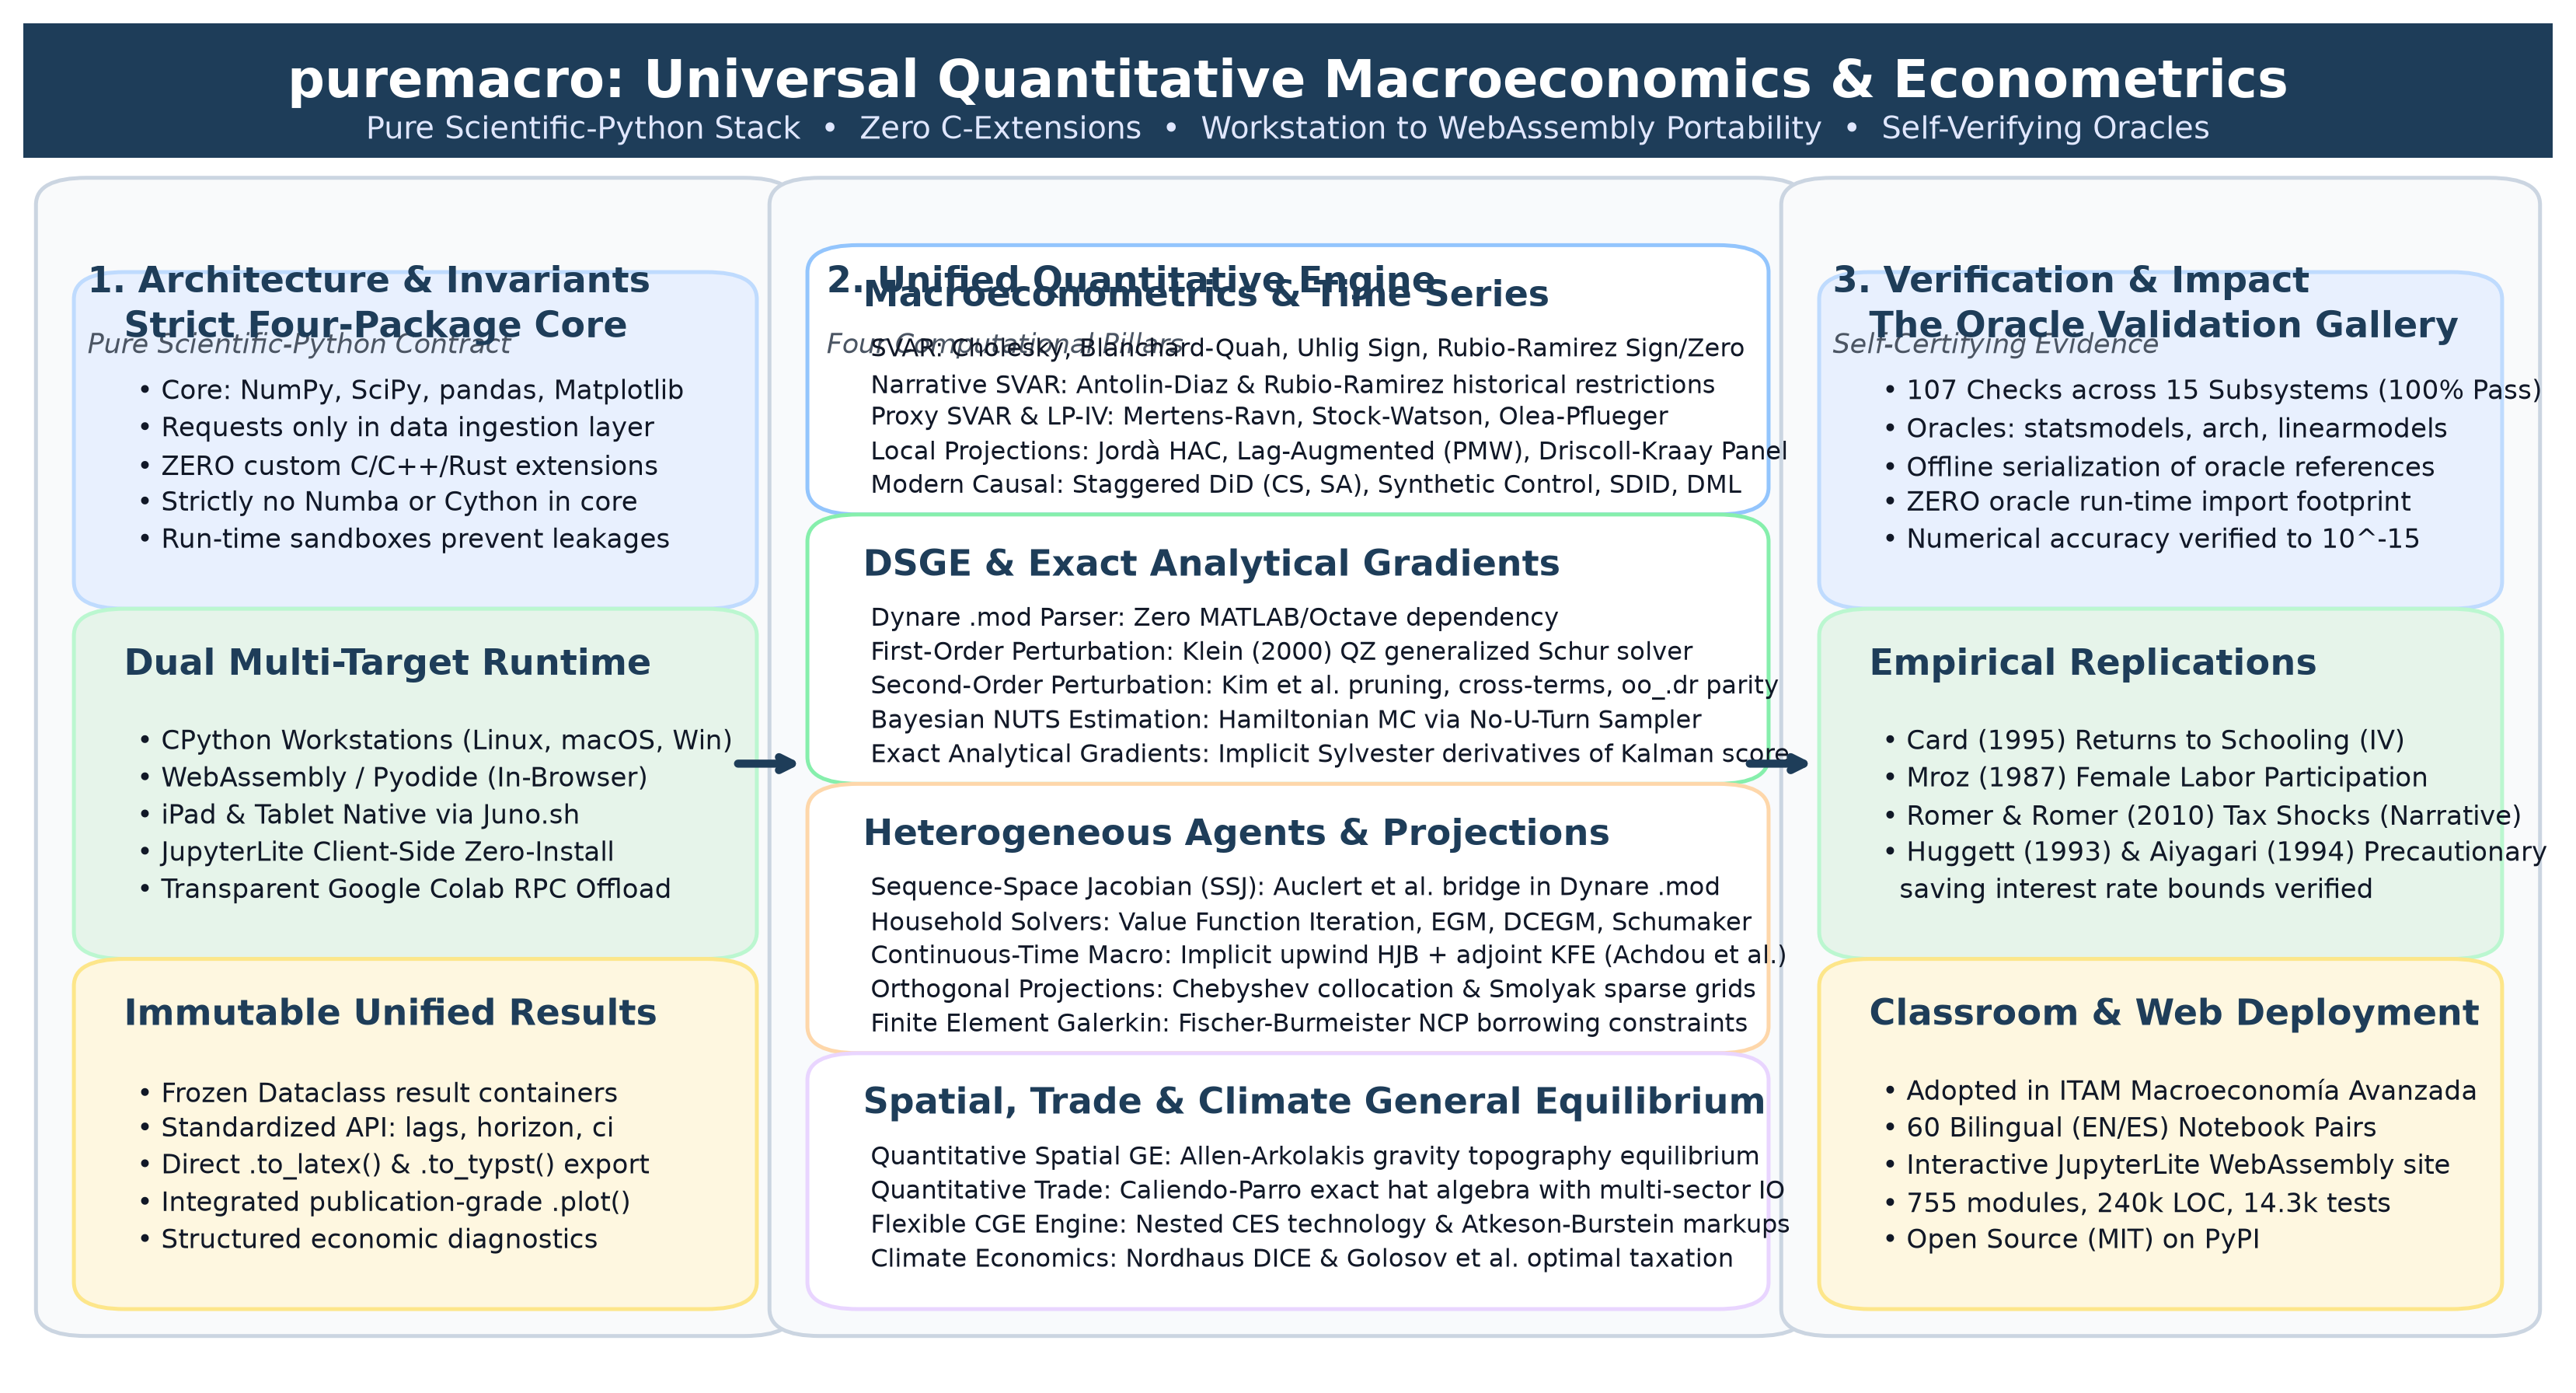
\includegraphics[width=\textwidth]{figures/graphical_abstract.png}
\caption{\textbf{Comprehensive Graphical Abstract of the \texttt{puremacro} Computational Ecosystem.} The diagram summarizes the architectural foundations, methodological engines, validation mechanisms, and deployment workflows. The left column outlines the strict four-package foundation (NumPy, SciPy, pandas, Matplotlib) and dual execution runtime (CPython and Pyodide WebAssembly). The center column displays the four primary computational pillars: structural macroeconometrics and causal inference, dynamic general equilibrium with exact analytical gradients, heterogeneous agents and continuous projections, and quantitative spatial and trade general equilibrium. The right column illustrates the self-certifying oracle validation gallery, landmark empirical replications, and zero-friction interactive web and classroom deployment.}
\label{fig:graphical_abstract}
\end{figure}

\clearpage
\tableofcontents
\clearpage

% --- Section 1: Introduction ---
\section{Introduction and the Computational Macroeconomics Trilemma}
\label{sec:introduction}

Applied macroeconomics and quantitative macroeconomic theory currently confront a profound technological challenge. While the discipline has experienced unprecedented methodological innovation over the past two decades—ranging from high-frequency identification of structural shocks and non-linear local projections to heterogeneous-agent New Keynesian (HANK) models and quantitative spatial gravity frameworks—the computational infrastructure supporting these advances remains severely fragmented. In contemporary research and graduate training, an applied economist typically must orchestrate four or five distinct software environments. Reduced-form time-series econometrics and volatility modeling frequently reside in specialized Python libraries such as \texttt{statsmodels} \citep{statsmodels2010} and \texttt{arch} \citep{arch}, or dedicated packages in R such as \texttt{vars} \citep{pfaff2008} and \texttt{lpirfs} \citep{adammer2019}. Meanwhile, linearized and higher-order dynamic stochastic general equilibrium (DSGE) modeling remains heavily anchored to Dynare \citep{dynare2024}, which operates within the proprietary MATLAB matrix laboratory or GNU Octave. Furthermore, heterogeneous-agent models and dynamic programming with continuous distributions are predominantly written in custom Fortran, C++, or Numba-accelerated Python codes \citep{auclert2021, carroll2018hark, quantecon2024}, while quantitative spatial and multi-sector trade general equilibrium models often rely on bespoke Julia or GAMS implementations \citep{caliendoparro2015, allenarkolakis2014}.

This computational balkanization imposes substantial friction across the research lifecycle. First, combining diverse packages forces researchers to manage disparate data structures, conflicting variable naming conventions, and incompatible parameter specifications, substantially elevating the cognitive overhead required to conduct empirical investigations. Second, the reliance on commercial platforms or packages with complex compiled C-extensions creates prohibitive barriers to scientific reproducibility. Empirical replication packages frequently break when installed on different operating systems or updated compiler toolchains, rendering long-term verification precarious. Third, this technological fragmentation proves particularly devastating in educational contexts. In advanced undergraduate and graduate macroeconomic courses, valuable instructional time is routinely squandered debugging local compiler errors, managing virtual environments, and resolving operating system incompatibilities across student laptops. Students operating on low-end hardware, locked-down institutional machines, or tablets are frequently excluded from engaging directly with modern quantitative tools.

The foundational challenge confronting the discipline can be conceptualized as the \emph{Computational Macroeconomics Trilemma}, which formalizes the historical trade-offs governing macroeconomic software design. Under this trilemma, existing computational frameworks have traditionally achieved at most two of three core scientific desiderata. The first desideratum is \emph{Methodological Breadth}, which demands an end-to-end computational surface encompassing structural vector autoregressions, micro-macro causal inference, nonlinear perturbation DSGE models, continuous projection algorithms, heterogeneous-agent sequence-space frameworks, and multi-sector spatial general equilibrium. The second desideratum is \emph{Universal Portability}, which guarantees that numerical code executes within tested tolerances identically across diverse computing environments—including standard CPython workstations, client-side WebAssembly browsers via Pyodide, and mobile tablet operating systems—without requiring compiled binary extensions, administrative privileges, or proprietary software licenses. The third desideratum is \emph{Numerical Verifiability}, which ensures rigorous, machine-precision certification against established econometric benchmarks and analytical solutions while preserving absolute autonomy from brittle external runtime dependencies.

The open-source library \texttt{puremacro} was conceived and engineered specifically to resolve this trilemma. Released under the permissive MIT license, \texttt{puremacro} provides a comprehensive computational engine for macroeconometrics and quantitative macroeconomics built entirely upon the foundational scientific-Python stack: NumPy \citep{numpy2020}, SciPy \citep{scipy2020}, pandas \citep{mckinney2010}, and Matplotlib \citep{hunter2007}. The software contains strictly zero compiled C, C++, Cython, or Rust extensions of its own, and has five mandatory runtime dependencies: NumPy, SciPy, pandas, Matplotlib and requests .

By adhering strictly to this pure-Python constraint, \texttt{puremacro} achieves universal browser-native portability. Through the WebAssembly-compiled Pyodide distribution \citep{pyodide}, the entire library executes client-side directly within any modern web browser or on tablet applications such as Juno for iOS. Users can solve second-order DSGE models, estimate structural VARs with narrative sign restrictions, simulate continuous-time HJB equations, and perform synthetic control analyses on an iPad without establishing an internet connection or installing a single local binary. To ensure numerical integrity without compromising portability, \texttt{puremacro} introduces an \emph{Oracle Architecture}, wherein reference outputs from established external packages (\texttt{statsmodels}, \texttt{arch}, \texttt{linearmodels}, and \texttt{esda}) are pre-computed offline and bundled as compact static test fixtures. A self-contained validation gallery executes 107 automated tests across 15 subsystems, verifying that \texttt{puremacro}'s native vectorized algorithms reproduce published benchmarks and oracle calculations to machine precision ($10^{-15}$) without importing the oracle packages into the runtime environment.

The remainder of this monograph is organized as follows. Section~\ref{sec:architecture} details the software architecture, the import invariant, the oracle verification framework, and the unified result object standard. Section~\ref{sec:macroeconometrics} presents the theoretical and numerical foundations of the structural macroeconometrics engine, encompassing vector autoregressions, modern identification schemes, and local projections. Section~\ref{sec:causal_nowcasting} outlines the micro-macro causal inference modules and mixed-frequency nowcasting systems. Section~\ref{sec:dsge} explores dynamic general equilibrium modeling, including native Dynare parsing, pruned second-order perturbations, and Bayesian NUTS estimation via exact analytical Kalman score gradients. Section~\ref{sec:heterogeneous_agents} develops the heterogeneous-agent suite, detailing the sequence-space Jacobian bridge and continuous-time HJB solvers. Section~\ref{sec:projections} covers continuous state-space projection methods on Chebyshev, Smolyak, and finite element bases. Section~\ref{sec:trade_spatial} presents quantitative trade and spatial general equilibrium models. Section~\ref{sec:validation} documents empirical verification, error bounds, and landmark replications. Section~\ref{sec:pedagogy} highlights pedagogical impact and interactive deployment, and Section~\ref{sec:conclusion} concludes with a strategic roadmap.

% --- Section 2: Software Architecture ---
\section{Software Architecture and Fundamental Invariants}
\label{sec:architecture}

The architectural philosophy of \texttt{puremacro} is governed by the principle that computational software should maximize long-term scientific reproducibility, operational transparency, and universal accessibility. Achieving these objectives within an extensive library spanning over 755 modules and 240,000 lines of Python code requires strict enforcement of structural invariants throughout the development lifecycle.

\begin{figure}[htbp]
\centering
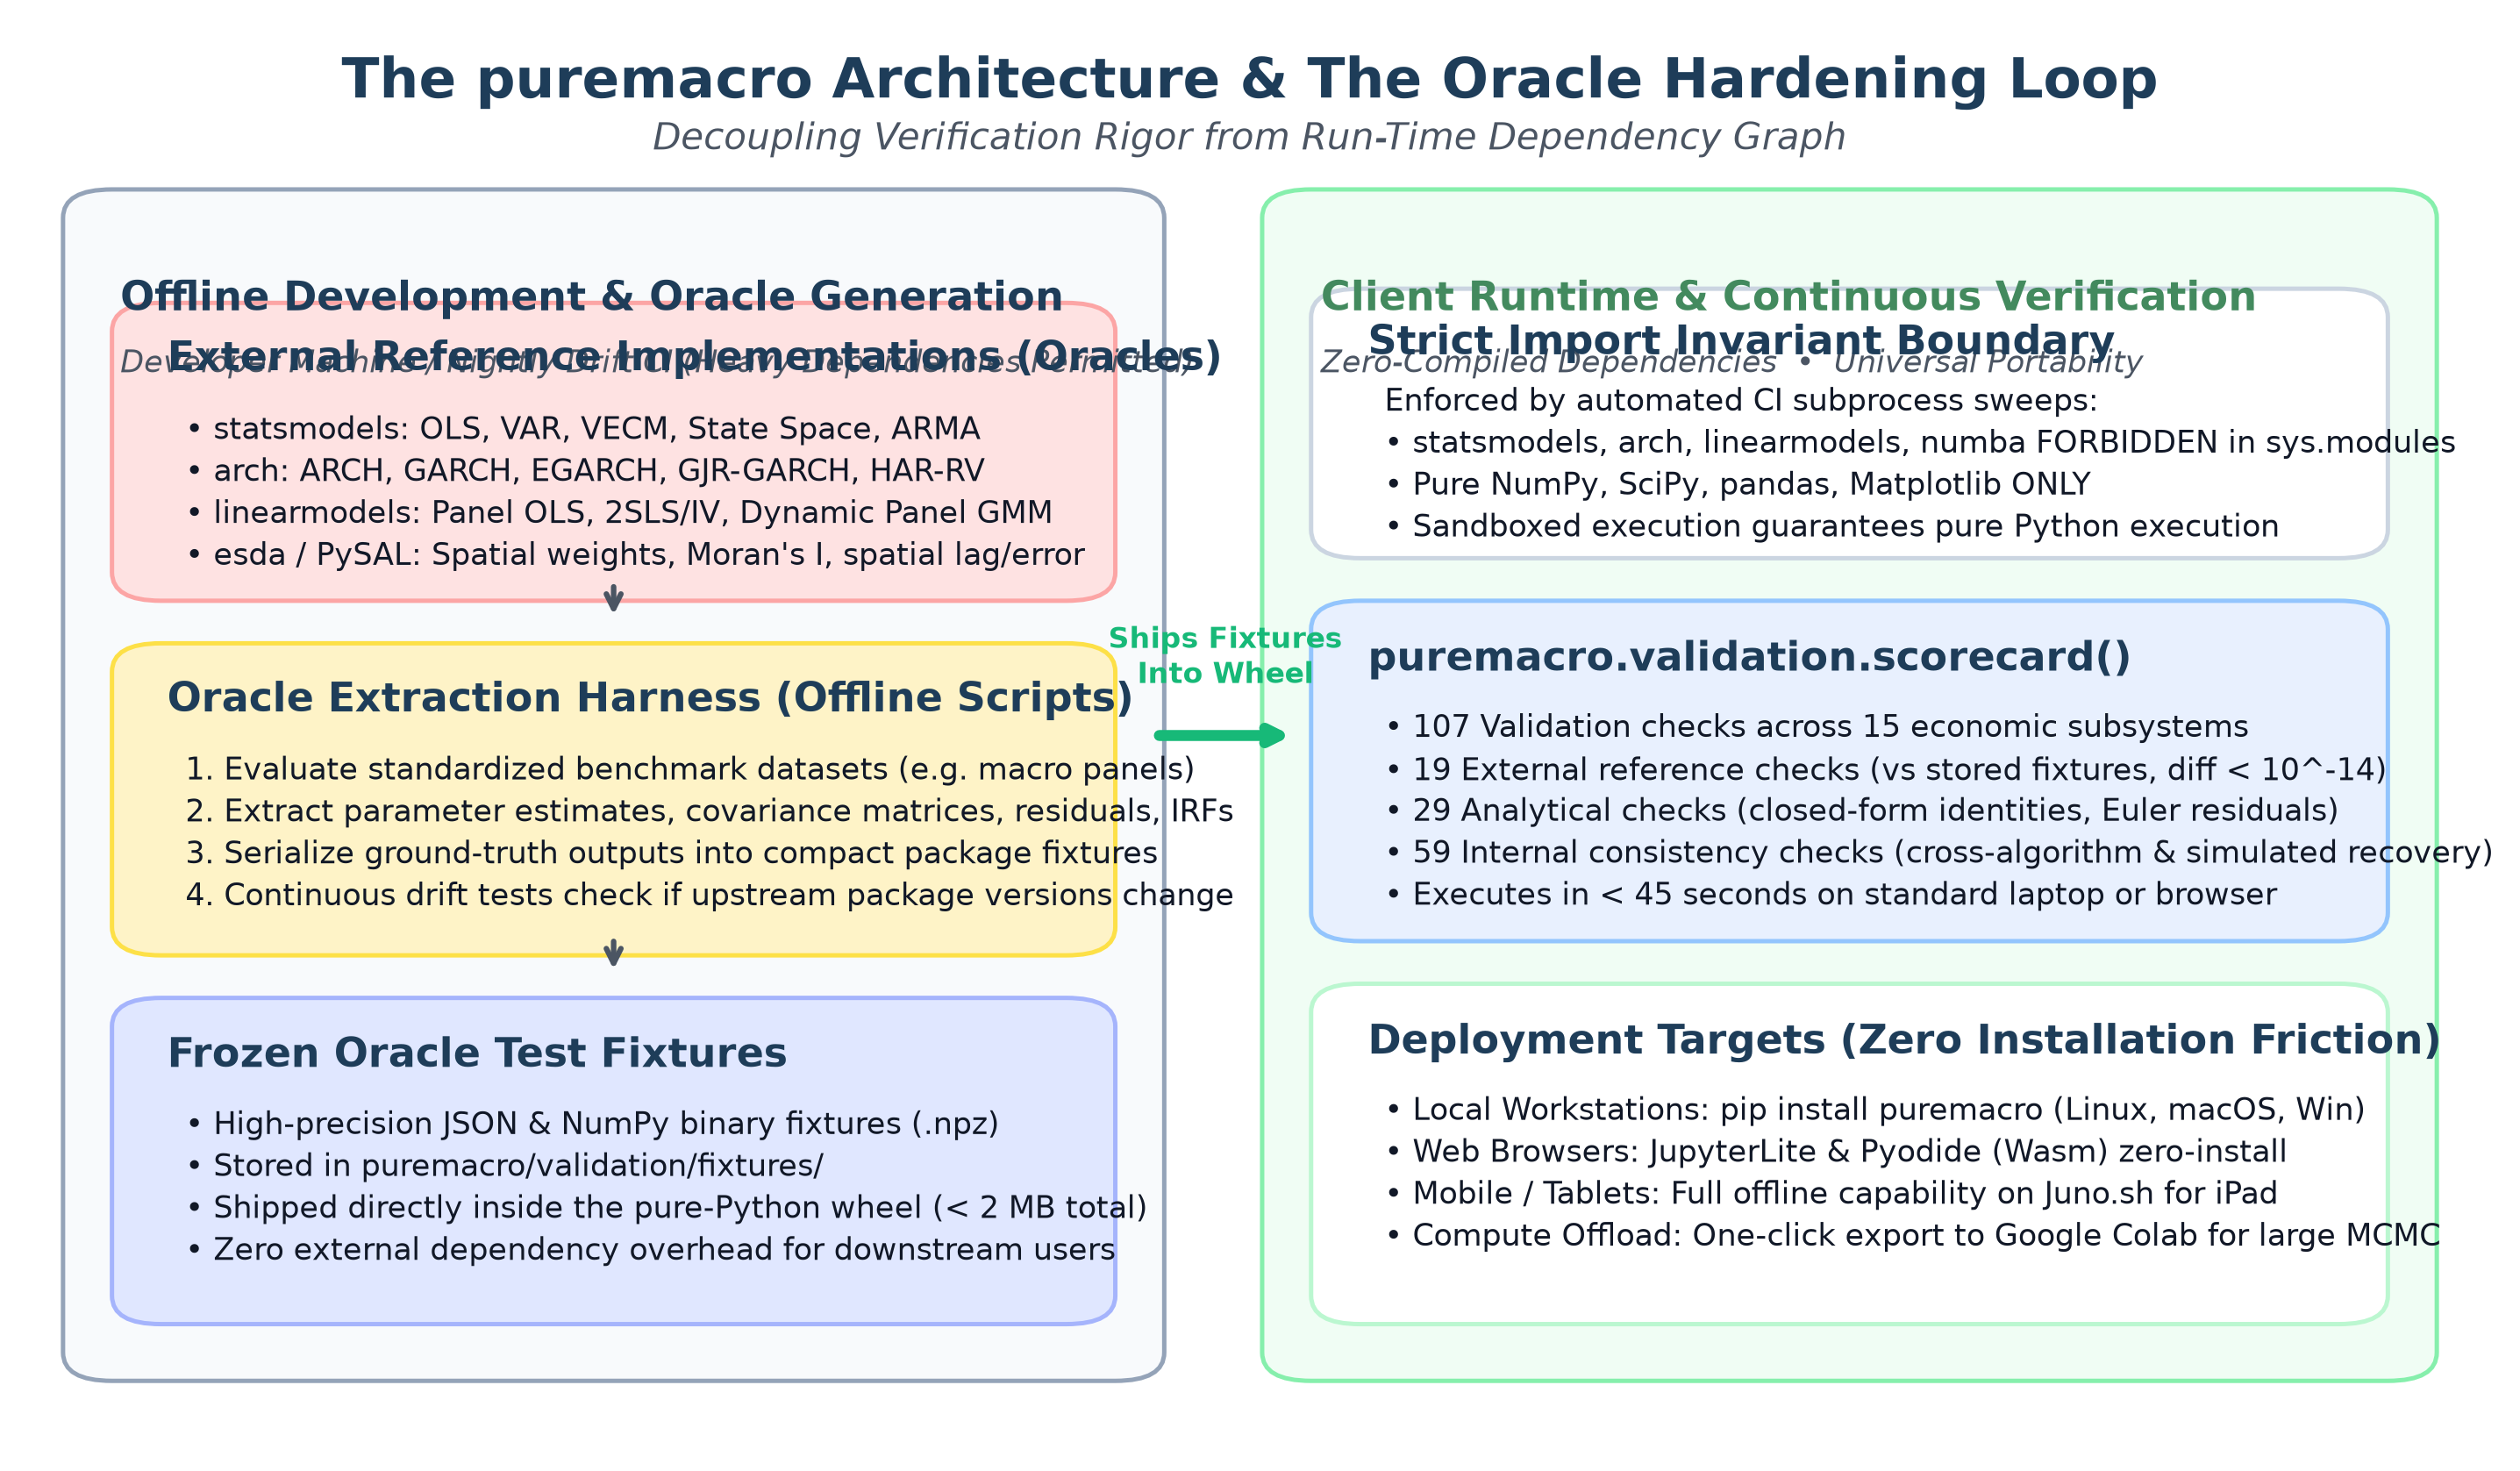
\includegraphics[width=\textwidth]{figures/fig_architecture_oracle.png}
\caption{\textbf{Software Architecture and the Oracle Hardening Loop in \texttt{puremacro}.} The schematic illustrates the decoupling between the offline verification environment and the client runtime. In the offline factory (left), established external packages (\texttt{statsmodels}, \texttt{arch}, \texttt{linearmodels}, and \texttt{esda}) compute oracle estimates on standardized macroeconomic datasets, serializing reference fixtures into compact package files. In the client environment (right), a strict import boundary forbids oracle libraries from entering the runtime. The self-contained gallery \texttt{puremacro.validation.scorecard()} illustrates a workflow; it does not certify all deployment targets.}
\label{fig:arch_oracle}
\end{figure}

\subsection{The Strict Four-Package Import Invariant}
The foundational invariant of \texttt{puremacro} dictates that library modules may import only NumPy, SciPy, pandas, and Matplotlib at module scope. All auxiliary functionality, such as Apache Parquet storage or specialized web-scraping utilities, is strictly optional and isolated behind lazy dynamic imports. Packages requiring custom compiled binaries—such as Numba, Cython, or external FORTRAN libraries—are entirely excluded from the numerical core.

To guarantee that this invariant is never violated during continuous development, the test suite implements two automated static and dynamic inspection sweeps. The first sweep programmatically traverses all 755 modules in the codebase, imports each module in isolation, and inspects the global interpreter table \texttt{sys.modules}. The test raises a fatal assertion failure if \texttt{statsmodels}, \texttt{linearmodels}, \texttt{arch}, \texttt{numba}, \texttt{cython}, or scraping dependencies have been loaded into interpreter memory. The second sweep executes the entire test suite inside an isolated subprocess whose environment variables deliberately block the importation of those external packages. Consequently, any inadvertent import leakage that would cause a failure on a constrained client machine or Pyodide browser sandbox immediately triggers a continuous integration failure on developer workstations.

\subsection{Decoupled Certification: The Oracle Architecture}
A central paradox in scientific software design is that establishing trust typically requires demonstrating agreement with established, peer-reviewed implementations; however, declaring those external implementations as formal runtime dependencies destroys portability and introduces severe dependency conflicts. \texttt{puremacro} resolves this tension through its \emph{Oracle Architecture}, depicted in Figure~\ref{fig:arch_oracle}.

During package development and release auditing, dedicated offline scripts execute external reference implementations—including \texttt{statsmodels} for vector autoregressions and state-space filters, \texttt{arch} for conditional heteroskedasticity, \texttt{linearmodels} for panel instrumental variables, and \texttt{esda} for spatial autocorrelation—across canonical benchmark datasets. The resulting point estimates, asymptotic covariance matrices, residual vectors, and impulse response trajectories are serialized into high-precision binary fixtures (\texttt{.npz} and structured JSON formats) stored within the \texttt{puremacro.validation.fixtures} directory. These fixtures ship directly inside the standard pure-Python wheel, adding less than 2 megabytes to the total distribution.

Frozen fixtures support offline comparisons without installing their generating packages. Live reference checks require those packages and apply only to the implemented comparisons.

\subsection{Immutable Result Containers and Publication-Ready Export}
To ensure reproducibility and facilitate scholarly workflow integration, \texttt{puremacro} eliminates the practice of returning unstructured tuples or raw NumPy arrays from estimators and solvers. All estimation routines return strongly typed, immutable frozen dataclasses adhering to a uniform API design.

Every result object encapsulates the complete estimation state, including estimated coefficient matrices, asymptotic or bootstrapped covariance structures, degrees of freedom, numerical convergence diagnostics, and underlying model specifications. Furthermore, all result containers expose a standardized suite of functional presentation methods designed to streamline academic dissemination. Invoking \texttt{.summary()} produces a formatted textual report detailing point estimates, standard errors, $t$-statistics, $p$-values, and confidence intervals matching standard econometric publishing conventions. Calling \texttt{.plot()} automatically renders publication-grade Matplotlib figures, generating impulse response fan charts with shaded confidence intervals, forecast error variance decompositions, or phase diagrams styled according to academic typography standards. For manuscript preparation, \texttt{.to\_latex()} emits complete, syntactically valid \LaTeX\ table markup formatted with \texttt{booktabs} horizontal rules, standard error parentheticals, and statistical significance indicators. Similarly, \texttt{.to\_typst()} generates native table definitions for the modern Typst typesetting engine, while \texttt{.to\_markdown()} outputs GitHub-flavored markdown tables for seamless integration into interactive computational notebooks, project documentation portals, and web applications.

\subsection{Dual Runtime Execution and Cloud Compute Offloading}
The elimination of compiled binaries enables a dual runtime operational model. On standard CPython interpreters running under Linux, macOS, or Windows, \texttt{puremacro} leverages underlying OpenBLAS, MKL, or Apple Accelerate linear algebra libraries via NumPy and SciPy, delivering high computational throughput. Simultaneously, because the entire codebase is pure Python, it runs natively inside the Pyodide WebAssembly virtual machine.

In resource-constrained environments, such as tablet browsers or mobile devices operating under strict memory caps, executing extensive Bayesian Markov Chain Monte Carlo simulations or high-dimensional bootstrap procedures can strain device capabilities. To address this, \texttt{puremacro} incorporates a transparent compute offloading architecture via \texttt{puremacro.runtime.colab}. This module can automatically package heavy computational tasks—such as a 10,000-draw No-U-Turn Sampler estimation of a medium-scale New Keynesian model—into a self-contained Jupyter notebook configured with Google Drive synchronization. The user can dispatch the computation to Google Colab's cloud infrastructure with a single function call, execute the simulation on remote hardware, and seamlessly deserialize the resulting compressed binary result cartridge (\texttt{.pmz}) back into their local tablet environment.

% --- Section 3: Structural Macroeconometrics ---
\section{Structural Macroeconometrics and Time-Series Analysis}
\label{sec:macroeconometrics}

Structural macroeconometrics seeks to uncover the causal effects of economic shocks on aggregate fluctuations by imposing theoretically grounded identification restrictions on reduced-form statistical models. \texttt{puremacro} provides a comprehensive, mathematically rigorous suite of vector autoregressive models and modern local projection estimators, standardizing interface conventions across all identification paradigms.

\begin{figure}[htbp]
\centering
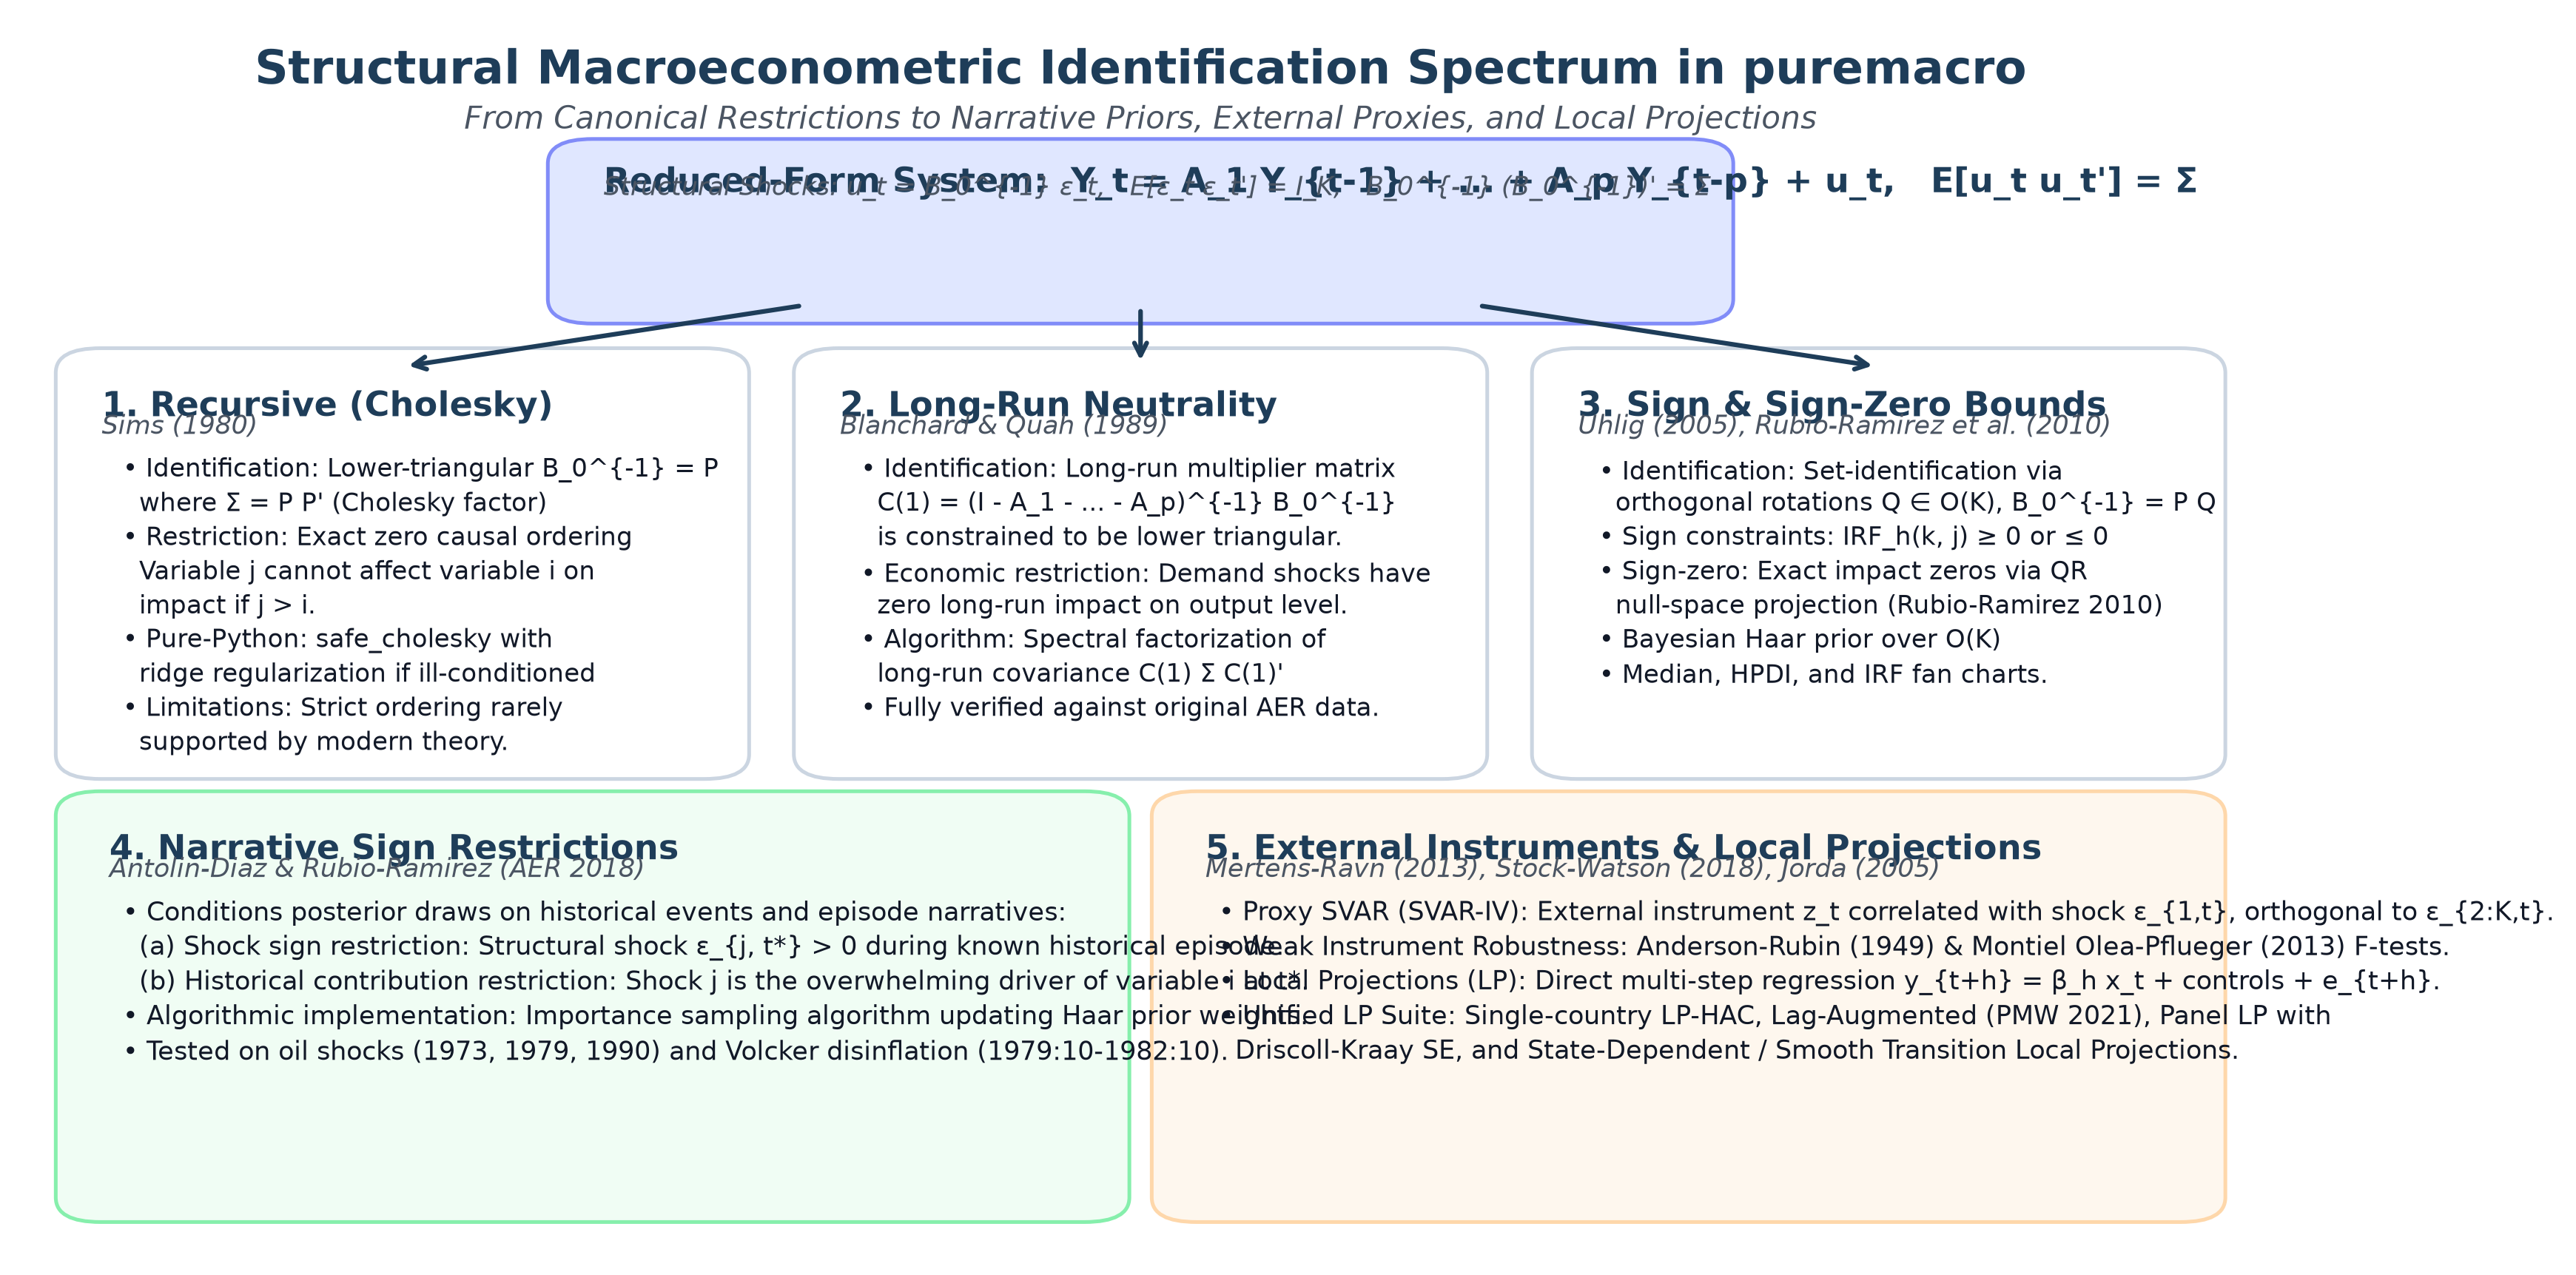
\includegraphics[width=\textwidth]{figures/fig_svar_identification.png}
\caption{\textbf{Structural Macroeconometric Identification Spectrum in \texttt{puremacro}.} The diagram maps the relationship between the reduced-form vector autoregression and five structural identification methodologies. The top container specifies the reduced-form VAR system and structural covariance decomposition. The lower cards contrast recursive Cholesky triangularization \citep{sims1980}, Blanchard-Quah long-run neutrality \citep{blanchardquah1989}, Uhlig and Rubio-Ram{\'i}rez sign and zero restrictions \citep{uhlig2005, rubioramirez2010}, Antol{\'i}n-D{\'i}az and Rubio-Ram{\'i}rez narrative restrictions \citep{antolindiaz2018}, and external proxy instruments and local projections \citep{mertensravn2013, stockwatson2018, jorda2005}.}
\label{fig:svar_spectrum}
\end{figure}

\subsection{Vector Autoregressions and Structural Identification}
Consider a covariance-stationary vector autoregressive process of order $p$, denoted VAR($p$):
\begin{equation}
    Y_t = c + \sum_{i=1}^p A_i Y_{t-i} + u_t, \quad u_t \sim \text{iid}(\mathbf{0}, \Sigma),
    \label{eq:reduced_var}
\end{equation}
where $Y_t$ is a $K \times 1$ vector of macroeconomic variables, $c$ is a vector of deterministic intercepts, $A_i$ are $K \times K$ coefficient matrices, and $u_t$ is the reduced-form innovation vector with symmetric positive-definite covariance matrix $\Sigma$. The structural representation relates reduced-form innovations $u_t$ to mutually orthogonal, economically meaningful structural shocks $\varepsilon_t$:
\begin{equation}
    u_t = B_0^{-1} \varepsilon_t, \quad \mathbb{E}[\varepsilon_t \varepsilon_t'] = I_K, \quad B_0^{-1} (B_0^{-1})' = \Sigma,
    \label{eq:structural_decomp}
\end{equation}
where $B_0^{-1}$ represents the structural impact matrix. Because $\Sigma$ contains $K(K+1)/2$ unique entries, while $B_0^{-1}$ contains $K^2$ parameters, the system is fundamentally under-identified, requiring $K(K-1)/2$ additional restrictions.

The library unifies the structural identification spectrum into a modular, consistent computational surface, illustrated in Figure~\ref{fig:svar_spectrum}. The most classical approach, recursive identification following \citet{sims1980}, imposes a causal ordering such that variable $j$ cannot affect variable $i$ contemporaneously if $j > i$. The impact matrix is obtained via the unique lower-triangular Cholesky factor $P$ satisfying $P P' = \Sigma$. The implementation in \texttt{puremacro} uses a regularized Cholesky factorization with eigenvalue floor clamping to guarantee numerical stability in empirical settings where high-dimensional macroeconomic covariance matrices approach singularity.

For long-run neutrality restrictions, \texttt{puremacro} implements the framework of \citet{blanchardquah1989}, wherein structural restrictions are imposed on the cumulative long-run multiplier matrix $C(1) = \left(I_K - \sum_{i=1}^p A_i\right)^{-1} B_0^{-1}$. Constraining $C(1)$ to be lower-triangular allows researchers to separate permanent supply disturbances from transitory demand shocks. The library evaluates $C(1)$ via direct spectral matrix inversion and factorizes $C(1) \Sigma C(1)'$ using numerically robust Cholesky decomposition, fully reproducing classical empirical findings.

Moving beyond exact zero restrictions, the library provides extensive support for agnostic sign and zero restrictions \citep{uhlig2005, rubioramirez2010}. Here, the identification space is parameterized by orthogonal rotation matrices $Q \in \mathcal{O}(K)$ such that $B_0^{-1} = P Q$, where $Q Q' = I_K$. Candidate rotation matrices are drawn uniformly over the Haar measure on the orthogonal group using QR decomposition of Gaussian random matrices. Sign restrictions on impulse response trajectories $\text{IRF}_h = \Phi_h P Q$ are audited across user-specified horizons. When exact contemporaneous zero restrictions are additionally imposed, \texttt{puremacro} implements the \citet{rubioramirez2010} algorithm, utilizing sequential Householder sub-space projections to restrict candidate columns of $Q$ to the null space of the zero constraints prior to drawing sign-consistent rotations.

To overcome the excessive breadth of sign-identified set estimates, \texttt{puremacro} incorporates the narrative sign restrictions methodology developed by \citet{antolindiaz2018}. This approach conditions posterior draws on historical narrative evidence, admitting two fundamental restriction types: narrative shock sign restrictions, which enforce that a structural shock was positive or negative during specific historical episodes, and narrative historical contribution restrictions, which require that a designated shock was the dominant contributor to an observed historical fluctuation. Posterior inference is executed via importance sampling that systematically reweights the uniform Haar prior conditional on narrative likelihood indicators. Finally, for settings where external proxy variables are available, the library provides proxy SVAR estimation \citep{mertensravn2013, stockwatson2018}, reporting the \citet{montieloleapflueger2013} effective $F$-statistic and \citet{andersonrubin1949} weak-instrument robust confidence sets.

\subsection{Local Projections and Inference Robustness}
As an alternative to vector autoregressions, \citet{jorda2005} introduced the method of local projections, which estimates impulse responses by fitting separate single-equation regressions for each forecast horizon $h \in \{0, 1, \dots, H\}$:
\begin{equation}
    y_{t+h} = \alpha_h + \beta_h x_t + \sum_{l=1}^p \gamma_{h, l}' w_{t-l} + \xi_{t+h},
    \label{eq:lp_basic}
\end{equation}
where $y_{t+h}$ is the response variable at horizon $h$, $x_t$ is the structural policy shock or treatment variable, and $w_{t-l}$ represents a vector of lagged control variables. The sequence of ordinary least squares estimates $\{\hat{\beta}_h\}_{h=0}^H$ traces the impulse response function directly without imposing the dynamic lag recursion inherent in VAR models.

Local projections exhibit substantial robustness against model misspecification in the underlying autoregressive lag structure; however, because the forecast errors $\xi_{t+h}$ inherently follow a moving average process of order $h$, the error terms are serially correlated. \texttt{puremacro} equips its local projection suite with rigorous covariance estimators. Single-country local projections (LP-HAC) employ heteroskedasticity and autocorrelation consistent standard errors following \citet{neweywest1987} with Bartlett kernel weights and automatic bandwidth selection. To resolve the bias-variance trade-off between structural VARs and local projections, the library incorporates lag-augmented local projections (LA-LP) based on the theorem of \citet{plagborgmollerwolf2021}, which proves that including sufficient lags of all endogenous variables guarantees asymptotic equivalence and valid inference even with unit roots. Furthermore, for longitudinal datasets, panel local projections incorporate \citet{driscollkraay1998} standard errors to account for cross-sectional spatial correlation and temporal persistence, while regime-switching local projections utilize logistic smooth transition functions to capture state-dependent shock transmission across business cycle phases.

\subsection{High-Frequency Identification and Volatility Modeling}
In financial macroeconomics, identifying monetary policy and macroeconomic news shocks requires isolating unexpected surprises occurring within tight intraday trading windows around central bank policy announcements. \texttt{puremacro} incorporates dedicated modules for processing high-frequency monetary surprise series, including the Gertler-Karadi and Nakamura-Steinsson surprise series, as well as unified volatility models.

The volatility engine provides pure-Python implementations of generalized autoregressive conditional heteroskedasticity (GARCH):
\begin{equation}
    r_t = \mu + \varepsilon_t, \quad \varepsilon_t = \sigma_t z_t, \quad z_t \sim \text{iid}(0, 1),
\end{equation}
\begin{equation}
    \sigma_t^2 = \omega + \alpha \varepsilon_{t-1}^2 + \beta \sigma_{t-1}^2,
    \label{eq:garch11}
\end{equation}
alongside asymmetric extensions including EGARCH and GJR-GARCH to capture leverage effects. For empirical settings linking high-frequency financial volatility with low-frequency macroeconomic fundamentals, the library implements GARCH-MIDAS \citep{engleghyselssohn2013}, which decomposes conditional variance into a short-run GARCH component and a long-run fundamental trend driven by macroeconomic indicators via beta-distributed polynomial lag filters.

% --- Section 4: Modern Causal Inference ---
\section{Micro-Macro Causal Inference and Nowcasting}
\label{sec:causal_nowcasting}

Modern empirical macroeconomics increasingly bridges aggregate time series with granular microeconomic panel data, leveraging quasi-experimental causal inference methods to evaluate policy reforms, tax changes, and subnational shocks. \texttt{puremacro} incorporates a complete suite of causal econometrics alongside dynamic factor models for real-time macroeconomic nowcasting.

\subsection{Modern Staggered Difference-in-Differences}
Recent econometric literature has demonstrated that traditional two-way fixed effects regressions fail in the presence of staggered treatment adoption and heterogeneous treatment effects, often yielding severely biased or negatively weighted policy estimates. To address this, \texttt{puremacro} implements the robust estimators of \citet{callaway2021} and \citet{sunabraham2021}.

The \citet{callaway2021} estimator identifies group-time average treatment effects $ATT(g, t)$ for cohorts first treated at time $g$:
\begin{equation}
    ATT(g, t) = \mathbb{E}\left[ Y_t - Y_{g-1} \mid G_g = 1 \right] - \mathbb{E}\left[ Y_t - Y_{g-1} \mid C = 1 \right],
    \label{eq:cs_att}
\end{equation}
where $G_g = 1$ denotes units treated in period $g$, and $C = 1$ denotes a clean comparison group composed either of never-treated units or not-yet-treated units. \texttt{puremacro} implements both outcome regression and doubly robust inverse-probability weighting schemes, providing automated aggregation of $ATT(g, t)$ into dynamic event-study trajectories and overall policy summaries with cluster-robust multiplier bootstrap standard errors.

\subsection{Synthetic Control and Synthetic Difference-in-Differences}
When evaluating policy interventions implemented in a single jurisdiction or aggregate unit, \texttt{puremacro} provides comparative case study methods that overcome the limitations of ad-hoc control selection. The synthetic control method of \citet{abadie2010} constructs an optimal convex combination of untreated donor units that minimizes the pre-treatment divergence between the treated unit and the donor pool. The donor weights $W^* = (w_2, \dots, w_{J+1})'$ are obtained by solving a constrained quadratic programming problem under non-negativity and sum-to-one restrictions. Statistical inference is conducted via systematic in-space and in-time placebo permutation tests, generating empirical $p$-values based on post-to-pre treatment mean squared prediction error ratios.

To enhance robustness in settings with substantial level differences between units, the library implements synthetic difference-in-differences (SDID) following \citet{arkhangelsky2021}. SDID generalizes the synthetic control framework by simultaneously estimating unit weights that balance pre-treatment trends and time weights that balance unexposed periods, while incorporating additive unit and time fixed effects. This dual regularization substantially reduces bias from unobserved additive confounders and improves efficiency relative to standard synthetic controls.

\subsection{Double / Debiased Machine Learning}
To estimate structural parameters in the presence of high-dimensional control variables without suffering from regularization bias, \texttt{puremacro.causal} implements Double/Debiased Machine Learning for the partially linear regression model \citep{chernozhukov2018}:
\begin{equation}
    Y = D \theta_0 + g_0(X) + U, \quad \mathbb{E}[U \mid D, X] = 0,
\end{equation}
\begin{equation}
    D = m_0(X) + V, \quad \mathbb{E}[V \mid X] = 0,
\end{equation}
where $D$ is the policy variable of interest, $X$ is a high-dimensional vector of controls, and $\theta_0$ is the structural parameter. The algorithm employs $K$-fold cross-fitting and constructs Neyman-orthogonal score functions $\psi(W; \theta, \eta) = (Y - \hat{g}(X) - \theta (D - \hat{m}(X))) (D - \hat{m}(X))$ using native regularized linear estimators, delivering $\sqrt{N}$-consistent and asymptotically normal inference for $\theta_0$.

\subsection{Mixed-Frequency Nowcasting and Dynamic Factor Models}
Central banks and financial institutions must monitor economic activity in real time, where indicators are sampled at disparate frequencies (monthly industrial production vs. quarterly GDP) and subject to publication lags that create an unbalanced ragged edge of data.

\texttt{puremacro.nowcast} implements the dynamic factor model of \citet{giannone2008} and \citet{banburamodugno2014}. The observable vector $y_t$ is modeled as driven by a small number of latent common factors $f_t$:
\begin{equation}
    y_t = \Lambda f_t + e_t, \quad e_t \sim \mathcal{N}(0, R),
\end{equation}
\begin{equation}
    f_t = A_1 f_{t-1} + \dots + A_p f_{t-p} + u_t, \quad u_t \sim \mathcal{N}(0, Q).
    \label{eq:dfm_state}
\end{equation}
To handle arbitrary patterns of missing data and ragged edges without discarding observations, the model is cast into state-space form and estimated using an expectation-maximization algorithm coupled with a vectorized Kalman smoother. Following \citet{banburamodugno2014}, the EM update steps evaluate conditional expectations of missing data points directly, enabling real-time news decomposition that attributes revisions in GDP forecasts to specific economic news releases.

% --- Section 5: DSGE Modeling ---
\section{Dynamic Stochastic General Equilibrium (DSGE) Modeling}
\label{sec:dsge}

Dynamic stochastic general equilibrium models constitute the core workhorse of modern quantitative macroeconomics and monetary policy analysis. Historically, solving and estimating DSGE models has required MATLAB/Octave workflows, including open-source Dynare. \texttt{puremacro} establishes a self-contained, native Python DSGE engine that parses Dynare \texttt{.mod} files, computes pruned higher-order perturbation solutions, and performs Bayesian estimation via Hamiltonian Monte Carlo using exact analytical likelihood gradients.

\begin{figure}[htbp]
\centering
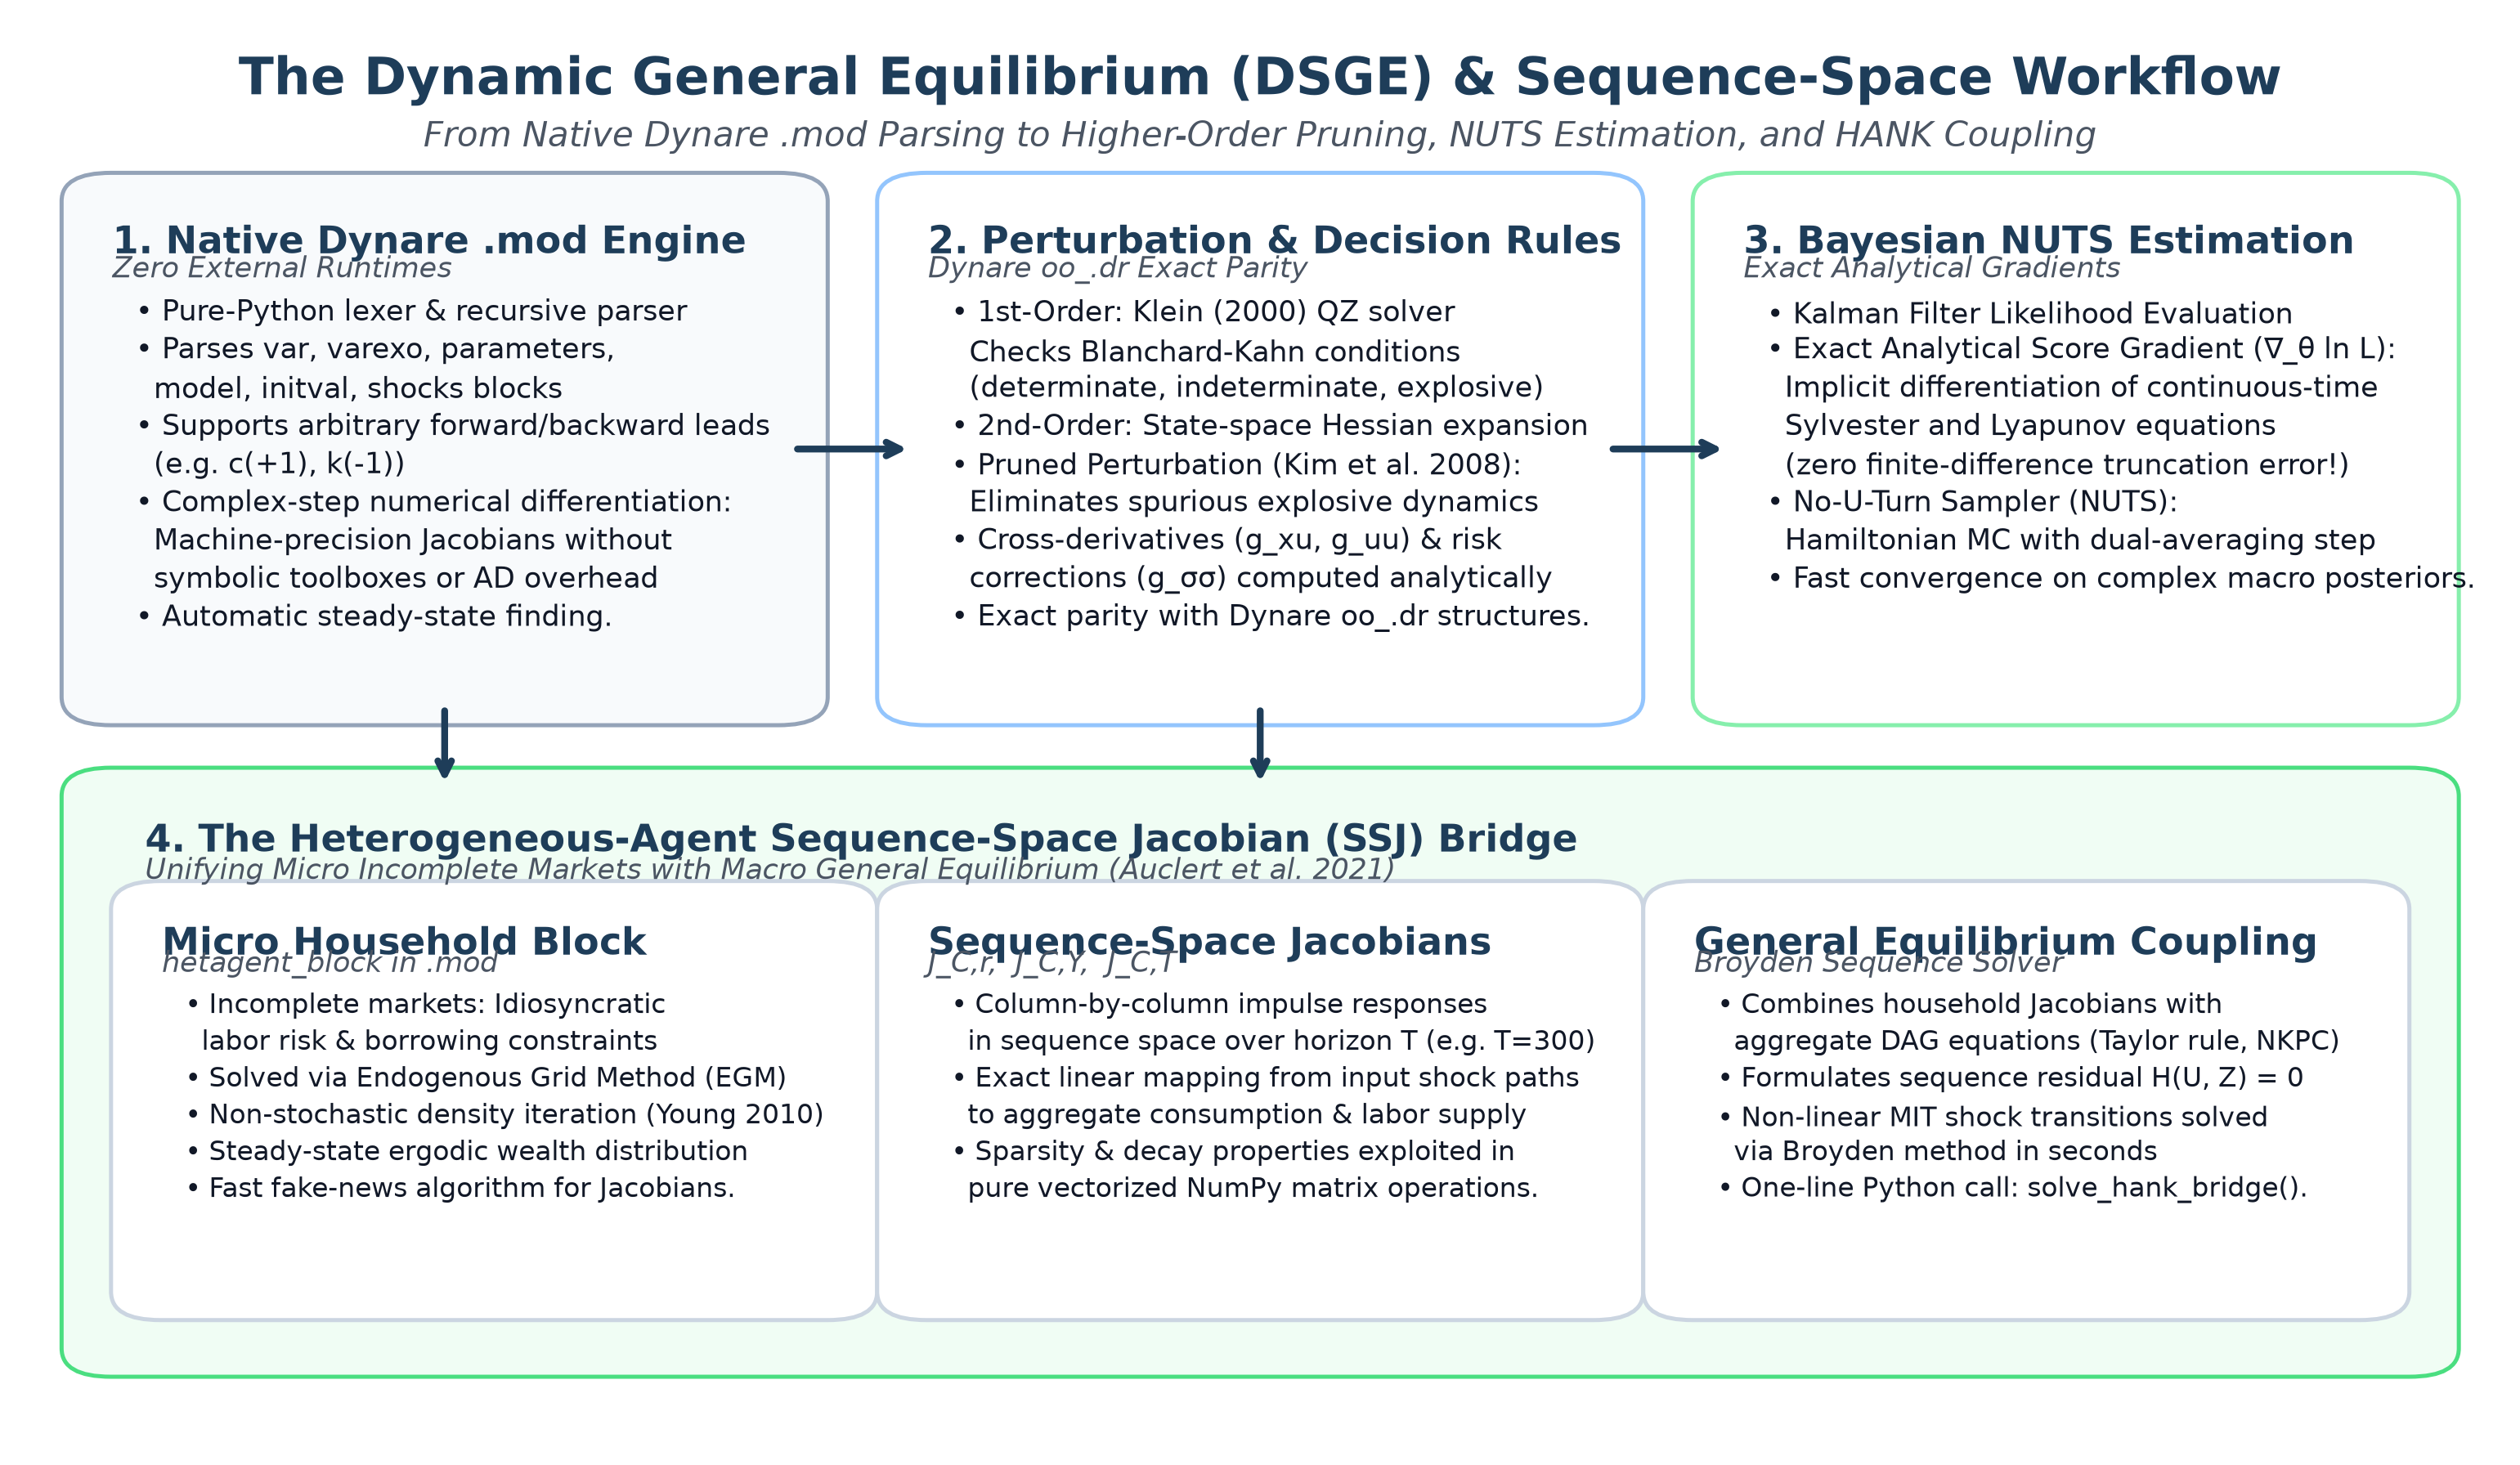
\includegraphics[width=\textwidth]{figures/fig_dsge_ssj_workflow.png}
\caption{\textbf{Integrated DSGE Perturbation, Bayesian NUTS Estimation, and Sequence-Space Jacobian Workflow.} The architecture encompasses four integrated stages: (1) native parsing of Dynare \texttt{.mod} syntax and complex-step Jacobian differentiation; (2) first-order Klein QZ solutions and second-order perturbation with Kim et al. pruning and risk corrections ($g_{\sigma\sigma}$); (3) Bayesian estimation via the No-U-Turn Sampler (NUTS) utilizing exact analytical Kalman likelihood score gradients ($\nabla_\theta \ln L$); and (4) coupling microeconomic heterogeneous-agent household blocks with aggregate DSGE market-clearing conditions via the Auclert et al. sequence-space Jacobian method.}
\label{fig:dsge_workflow}
\end{figure}

\subsection{Native Dynare Parser and Complex-Step Differentiation}
\texttt{puremacro.dsge} features a native lexer and recursive-descent parser capable of reading Dynare \texttt{.mod} files directly. The parser interprets standard declaration blocks, including \texttt{var}, \texttt{varexo}, \texttt{parameters}, \texttt{model}, \texttt{initval}, and \texttt{shocks}, resolving arbitrary dynamic lead-lag relationships (such as $c_{t+1}$ represented as \texttt{c(+1)} and $k_{t-1}$ as \texttt{k(-1)}).

A major bottleneck in non-symbolic DSGE solvers is the accumulation of numerical truncation errors during numerical differentiation of non-linear equilibrium equations $f(y_{t+1}, y_t, y_{t-1}, u_t; \theta) = 0$. While standard finite differencing suffers from $O(\epsilon)$ cancellation errors, \texttt{puremacro} utilizes the complex-step derivative approximation:
\begin{equation}
    \frac{\partial f_i(x)}{\partial x_j} = \frac{\text{Im}\left[ f_i(x + i h e_j) \right]}{h} + O(h^2),
    \label{eq:complex_step}
\end{equation}
where $h = 10^{-20}$ and $e_j$ is the $j$-th unit basis vector. Because the complex-step formulation involves no subtraction in the numerator, it is entirely immune to catastrophic cancellation, providing accurate first derivatives for complex-safe functions; finite-difference higher derivatives retain truncation and rounding error.

\subsection{First- and Second-Order Perturbation with Dynare Parity}
Given the equilibrium system $\mathbb{E}_t [ f(y_{t+1}, y_t, y_{t-1}, u_t) ] = 0$, the first-order approximation around the deterministic steady state $(\bar{y}, \mathbf{0})$ yields a linear rational expectations system:
\begin{equation}
    A \mathbb{E}_t \hat{y}_{t+1} + B \hat{y}_t + C \hat{y}_{t-1} + D u_t = 0.
\end{equation}
\texttt{puremacro} solves this system using the generalized Schur (QZ) decomposition method of \citet{klein2000}, automatically checking the \citet{blanchardkahn1980} rank and order conditions to classify the model as uniquely determinate, indeterminate, or explosive. The policy decision rules take the form:
\begin{equation}
    \hat{y}_t = g_x \hat{s}_{t-1} + g_u u_t,
\end{equation}
which can be compared against supplied Dynare decision-rule references. Agreement must be assessed per model and field.

For welfare analysis, term premia, and precautionary behavior, linear approximations are insufficient. \texttt{puremacro} implements second-order perturbation approximations:
\begin{equation}
    \hat{y}_t = g_x \hat{s}_{t-1} + g_u u_t + \frac{1}{2} G_{xx} (\hat{s}_{t-1} \otimes \hat{s}_{t-1}) + \frac{1}{2} G_{uu} (u_t \otimes u_t) + G_{xu} (\hat{s}_{t-1} \otimes u_t) + \frac{1}{2} g_{\sigma\sigma} \sigma^2,
    \label{eq:second_order}
\end{equation}
where $g_{\sigma\sigma}$ represents the endogenous risk correction shifting the stochastic steady state away from the deterministic baseline. To prevent spurious explosive dynamics that frequently plague unpruned higher-order simulations, \texttt{puremacro} strictly implements the pruning algorithm of \citet{kim2008}, decomposing state trajectories into first-order and second-order components that guarantee stationary simulated paths.

\subsection{Bayesian Estimation via NUTS and Exact Analytical Score Gradients}
Estimating DSGE models via Bayesian methods requires evaluating the Gaussian log-likelihood $\ln L(\theta \mid Y_{1:T})$ via the Kalman filter:
\begin{equation}
    \ln L(\theta \mid Y_{1:T}) = -\frac{T K}{2} \ln(2\pi) - \frac{1}{2} \sum_{t=1}^T \left( \ln |F_t| + v_t' F_t^{-1} v_t \right),
    \label{eq:kalman_loglik}
\end{equation}
where $v_t = Y_t - Z \hat{s}_{t \mid t-1}$ represents the one-step-ahead forecast error and $F_t = Z P_{t \mid t-1} Z' + H$ is its covariance matrix. In existing packages, sampling from the posterior distribution $p(\theta \mid Y_{1:T}) \propto L(\theta \mid Y_{1:T}) p(\theta)$ relies heavily on the Random Walk Metropolis-Hastings algorithm, which suffers from slow exploration and poor scalability in high-dimensional parameter spaces.

To achieve superior sampling efficiency, \texttt{puremacro} implements the No-U-Turn Sampler, an adaptive Hamiltonian Monte Carlo algorithm \citep{hoffman2014}. Efficient Hamiltonian dynamics require the gradient of the log-posterior $\nabla_\theta \ln p(\theta \mid Y_{1:T}) = \nabla_\theta \ln L(\theta) + \nabla_\theta \ln p(\theta)$. While finite-difference approximations of Kalman likelihood gradients are notoriously noisy and computationally expensive, \texttt{puremacro} implements exact analytical score gradients $\nabla_\theta \ln L$.

The analytical gradient is derived by applying the chain rule through the steady-state Kalman filter recursions:
\begin{equation}
    \frac{\partial \ln L}{\partial \theta_j} = -\frac{1}{2} \sum_{t=1}^T \left[ \text{tr}\left( F^{-1} \frac{\partial F}{\partial \theta_j} \right) + 2 v_t' F^{-1} \frac{\partial v_t}{\partial \theta_j} - v_t' F^{-1} \frac{\partial F}{\partial \theta_j} F^{-1} v_t \right].
\end{equation}
Computing $\partial F / \partial \theta_j$ requires the derivative of the steady-state state error covariance $P_\infty$ satisfying the Discrete Algebraic Riccati Equation (DARE). By differentiating the DARE with respect to parameter $\theta_j$, \texttt{puremacro} demonstrates that $\partial P_\infty / \partial \theta_j$ satisfies a continuous-matrix Sylvester equation:
\begin{equation}
    \tilde{A} \left( \frac{\partial P_\infty}{\partial \theta_j} \right) \tilde{A}' - \frac{\partial P_\infty}{\partial \theta_j} + \tilde{Q}_j = 0,
    \label{eq:sylvester}
\end{equation}
where $\tilde{A}$ is the closed-loop transition matrix and $\tilde{Q}_j$ collects structural derivative terms. \texttt{puremacro} solves these matrix Sylvester systems using vectorized Bartels-Stewart algorithms in SciPy, delivering exact analytical likelihood gradients to machine precision. Consequently, the NUTS sampler achieves rapid trajectory acceptance, high effective sample sizes, and reliable posterior convergence across benchmark medium-scale DSGE models.

% --- Section 6: Heterogeneous-Agent Macroeconomics ---
\section{Heterogeneous-Agent Macroeconomics and Sequence Space}
\label{sec:heterogeneous_agents}

The frontiers of macroeconomic research increasingly emphasize models with rich household and firm heterogeneity, incomplete insurance markets, and idiosyncratic income risk. \texttt{puremacro} bridges microeconomic heterogeneous-agent blocks with aggregate general equilibrium using two advanced paradigms: the Sequence-Space Jacobian method and continuous-time partial differential equations.

\subsection{Microeconomic Household Optimization and Ergodic Distributions}
The microeconomic foundation of heterogeneous-agent models consists of households optimizing consumption and wealth accumulation subject to idiosyncratic labor productivity risk and uninsurable borrowing constraints \citep{huggett1993, aiyagari1994}. The household problem satisfies the Bellman equation:
\begin{equation}
    v(a, s) = \max_{c, a'} \left\{ u(c) + \beta \sum_{s'} \pi(s' \mid s) v(a', s') \right\},
\end{equation}
subject to:
\begin{equation}
    c + a' = (1 + r) a + w s + T, \quad a' \ge \underline{a},
\end{equation}
where $a$ is asset holdings, $s$ is Markovian labor productivity, $r$ is the real interest rate, $w$ is the real wage, and $\underline{a}$ denotes the borrowing limit.

The computational module \texttt{puremacro.vfi} provides an integrated suite of policy function solvers designed to eliminate optimization bottlenecks. For standard concave consumption problems, the library implements the Endogenous Grid Method \citep{carroll2006}, which inverts the first-order Euler equation to map future asset choices directly to current policy values without numerical rootfinding. When households confront discrete decisions—such as occupational choice, retirement timing, or default—the module deploys Discrete-Continuous EGM \citep{iskhakov2017}, incorporating an analytical upper-envelope filter that prunes suboptimal policy branches arising from non-concave value functions. To track the evolution of cross-sectional distributions over time, \texttt{puremacro} implements the non-stochastic forward density iteration framework of \citet{young2010}, updating asset-productivity distributions over fine piecewise-linear grids to compute invariant ergodic measures without Monte Carlo simulation variance.

\subsection{The Sequence-Space Jacobian (SSJ) Bridge}
To analyze aggregate shocks and general equilibrium dynamics in heterogeneous-agent New Keynesian models, \texttt{puremacro} incorporates the Sequence-Space Jacobian framework of \citet{auclert2021}.

Rather than relying on state-space master equations that suffer from severe dimensionality curses, the SSJ method linearizes the heterogeneous-agent economy around its stationary equilibrium directly in the space of infinite sequences. Let $\mathbf{Z} = \{Z_t\}_{t=0}^\infty$ represent aggregate input price paths (such as interest rates, wages, and transfers) and $\mathbf{X} = \{X_t\}_{t=0}^\infty$ represent aggregate output decisions (such as consumption and labor supply). The linearized household response satisfies:
\begin{equation}
    d\mathbf{X} = \mathcal{J}_{\mathbf{X}, \mathbf{Z}} \, d\mathbf{Z},
\end{equation}
where $\mathcal{J}_{\mathbf{X}, \mathbf{Z}} = \left[ \frac{\partial X_t}{\partial Z_s} \right]_{t, s \ge 0}$ is the sequence-space Jacobian matrix. \texttt{puremacro} implements the fake news algorithm \citep{auclert2021}, which computes these extensive $T \times T$ Jacobian matrices in a fraction of a second by decomposing impulse responses into prediction vectors and distribution transition operators.

Remarkably, \texttt{puremacro} integrates this machinery directly into Dynare syntax via the novel \texttt{hetagent\_block;} declaration inside \texttt{.mod} files. The parser automatically extracts the household block, solves the stationary steady state, computes the sequence-space Jacobians, and couples them with aggregate block equations (e.g., Phillips curves and monetary policy rules). The general equilibrium transition paths following unexpected aggregate shocks (e.g., a monetary tightening or fiscal expansion) are solved via sequence-space Broyden rootfinding in seconds, achieving full HANK capabilities within a pure-Python library.

\subsection{Continuous-Time Macroeconomics: Upwind HJB-KFE Solvers}
For continuous-time heterogeneous-agent economies, \texttt{puremacro} implements the monotone finite-difference framework of \citet{achdou2022}. The household's stationary value function satisfies the Hamilton-Jacobi-Bellman partial differential equation:
\begin{equation}
    \rho v(a, y_i) = \max_{c} \left\{ u(c) + v_a(a, y_i) (r a + w y_i - c) \right\} + \sum_{j \neq i} \lambda_{ij} \left[ v(a, y_j) - v(a, y_i) \right],
    \label{eq:hjb_continuous}
\end{equation}
subject to $a \ge \underline{a}$. To guarantee numerical stability and preserve the viscosity solution, the drift derivative $v_a(a, y_i)$ is discretized using an implicit upwind finite-difference scheme. When the savings drift $s_i(a) = r a + w y_i - c$ is positive, forward differences are employed; when negative, backward differences are utilized.

This upwind discretization generates a sparse, strictly diagonally dominant $M$-matrix, ensuring that the implicit time-stepping algorithm converges unconditionally. The corresponding stationary wealth distribution $g(a, y_i)$ is determined by the adjoint Kolmogorov Forward Equation:
\begin{equation}
    -\frac{\partial}{\partial a} \left[ s_i(a) g(a, y_i) \right] - \sum_{j} \lambda_{ji} g(a, y_j) = 0, \quad \sum_i \int_{\underline{a}}^\infty g(a, y_i) \, da = 1.
\end{equation}
In discrete form, this system simplifies to $A' \mathbf{g} = \mathbf{0}$, which \texttt{puremacro} solves via sparse LU factorization in pure SciPy, completing the continuous-time general equilibrium loop with exceptional numerical fidelity.

% --- Section 7: Continuous Projection Methods ---
\section{Continuous State-Space Projection Methods}
\label{sec:projections}

While perturbation methods provide local approximations around a deterministic steady state, highly non-linear economic problems—such as models with occasionally binding borrowing constraints, large structural shifts, or persistent uncertainty—demand global solution methods. \texttt{puremacro.vfi} provides an extensive suite of continuous projection algorithms, illustrated in Figure~\ref{fig:vfi_projections}.

\begin{figure}[htbp]
\centering
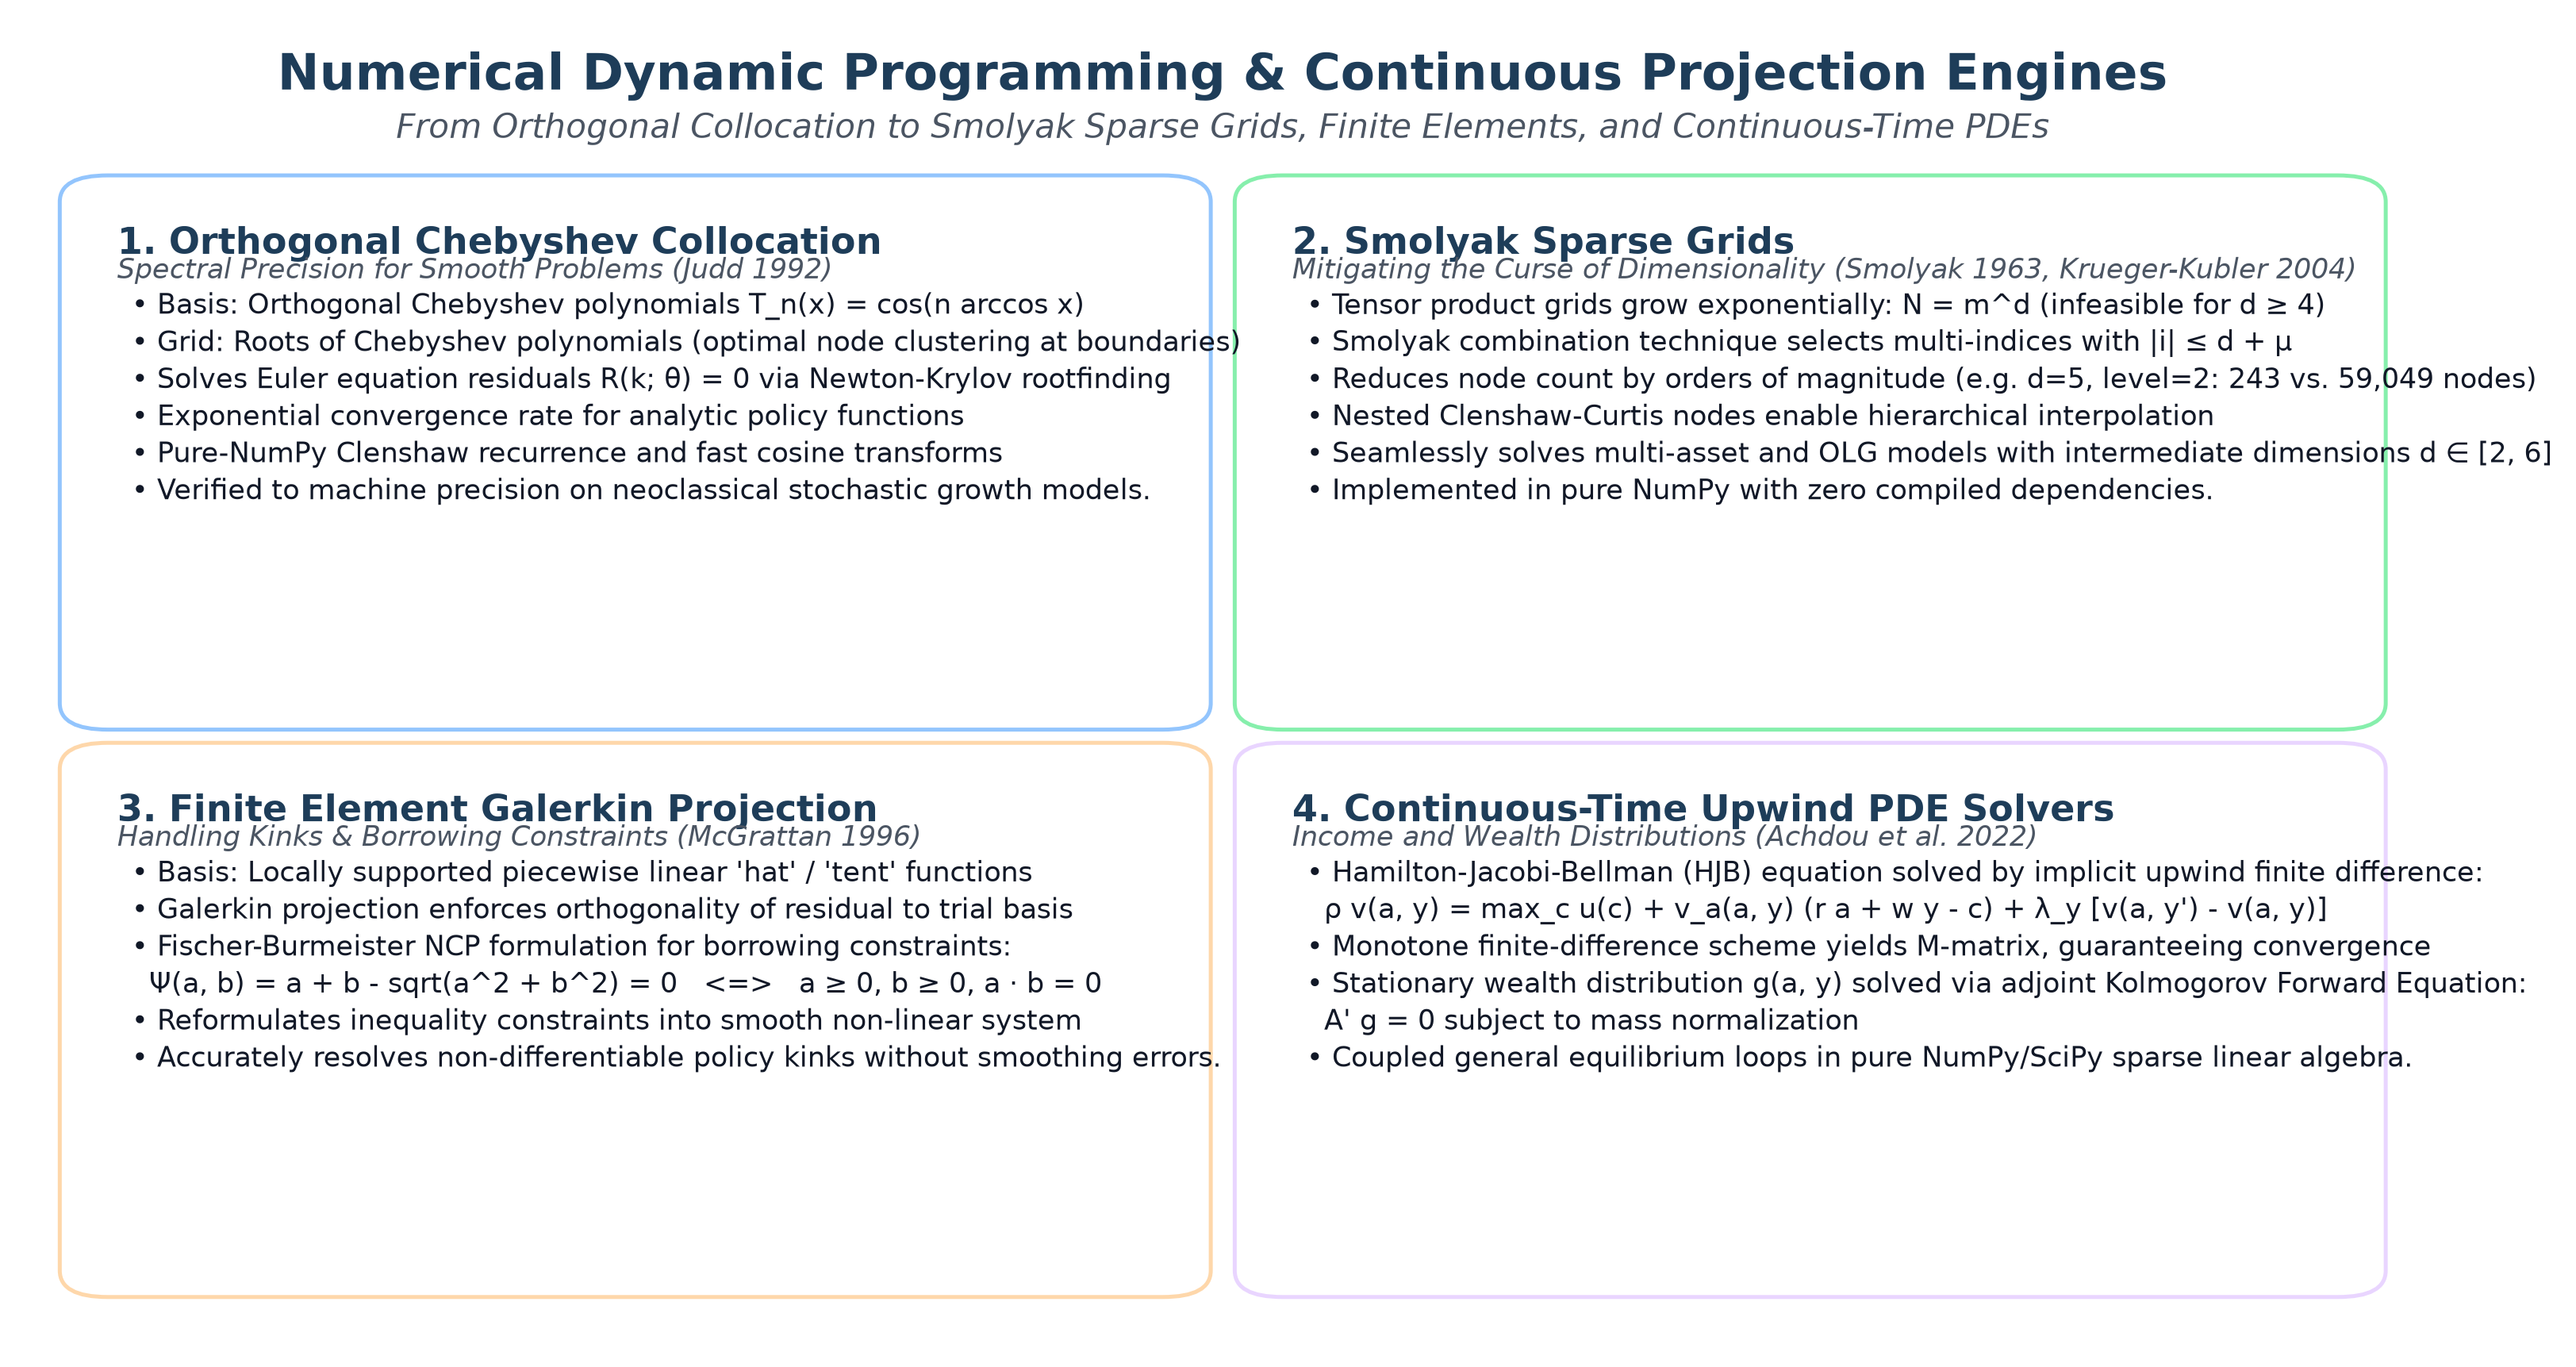
\includegraphics[width=\textwidth]{figures/fig_vfi_projections.png}
\caption{\textbf{Continuous State-Space Projection and Numerical Dynamic Programming Engines in \texttt{puremacro}.} The four quadrants contrast complementary numerical approaches: (1) orthogonal Chebyshev polynomial collocation on smooth problems \citep{judd1992}; (2) Smolyak multidimensional sparse grid interpolation mitigating the curse of dimensionality \citep{smolyak1963, kruegerkubler2004}; (3) finite element Galerkin projection with Fischer-Burmeister NCP complementarity for non-differentiable borrowing kinks \citep{mcgrattan1996}; and (4) continuous-time implicit upwind PDE solvers for stationary wealth distributions \citep{achdou2022}.}
\label{fig:vfi_projections}
\end{figure}

\subsection{Orthogonal Chebyshev Collocation}
Following \citet{judd1992}, spectral projection methods approximate unknown policy or value functions using linear combinations of orthogonal basis polynomials. In a neoclassical growth model with capital state $k \in [\underline{k}, \bar{k}]$, the policy function for consumption $c(k)$ is approximated as:
\begin{equation}
    c_N(k) = \sum_{j=0}^{N-1} \gamma_j T_j(\phi(k)),
\end{equation}
where $T_j(x) = \cos(j \arccos(x))$ is the Chebyshev polynomial of degree $j$, and $\phi: [\underline{k}, \bar{k}] \to [-1, 1]$ is an affine coordinate mapping. Collocation nodes are chosen as the Chebyshev roots $x_i = -\cos\left(\frac{2i - 1}{2N} \pi\right)$, which optimize node clustering near boundaries to eliminate the Runge phenomenon.

The projection coefficients $\bm{\gamma} = (\gamma_0, \dots, \gamma_{N-1})'$ are determined by enforcing that the Euler equation residual:
\begin{equation}
    \mathcal{R}(k_i; \bm{\gamma}) \equiv u'(c_N(k_i)) - \beta \mathbb{E}\left[ u'(c_N(k')) (f'(k') + 1 - \delta) \right] = 0,
\end{equation}
is required to fall below the requested tolerance at the $N$ fitting nodes. This does not certify off-grid accuracy. \texttt{puremacro} solves this non-linear residual system via Broyden or Newton-Krylov algorithms utilizing Clenshaw recurrence in vectorized NumPy, achieving exponential convergence rates for analytic policy functions.

\subsection{Smolyak Sparse Grids and Dimensionality Mitigation}
In multi-state macroeconomic models (e.g., multi-country models, heterogeneous capital assets, or overlapping generations economies with state dimension $d \ge 3$), standard tensor-product polynomial grids succumb to the curse of dimensionality, where the required grid nodes grow exponentially as $N = m^d$.

To render continuous projections tractable for intermediate dimensions $d \in [2, 6]$, \texttt{puremacro} implements the Smolyak sparse grid interpolation algorithm \citep{smolyak1963, kruegerkubler2004}. Let $U^i$ denote a one-dimensional interpolation operator of order $i$. The Smolyak interpolation operator $A(q, d)$ of approximation level $\mu = q - d$ is formulated as a linear combination of tensor products over sparse multi-indices $\mathbf{i} = (i_1, \dots, i_d)$:
\begin{equation}
    A(q, d) = \sum_{q - d + 1 \le |\mathbf{i}| \le q} (-1)^{q - |\mathbf{i}|} \binom{d - 1}{q - |\mathbf{i}|} \left( U^{i_1} \otimes \dots \otimes U^{i_d} \right),
    \label{eq:smolyak}
\end{equation}
where $|\mathbf{i}| = \sum_{j=1}^d i_j$. By employing nested Clenshaw-Curtis quadrature nodes, \texttt{puremacro} achieves dramatic node reductions; for example, in a five-dimensional model ($d=5$) at level $\mu=2$, the Smolyak grid requires only 243 nodes, compared to 59,049 nodes required by an equivalent full tensor product grid, unlocking high-dimensional continuous policy solutions within a pure scientific-Python framework.

\subsection{Finite Element Galerkin Projection and Fischer-Burmeister Complementarity}
When macroeconomic policy functions exhibit sharp kinks or non-differentiable boundaries—most notably due to occasionally binding borrowing constraints $a' \ge \underline{a}$—global polynomial approximations suffer from Gibbs oscillations and poor convergence. \texttt{puremacro} addresses this through finite element Galerkin methods \citep{mcgrattan1996}.

The continuous asset domain is partitioned into local sub-elements, and policy functions are spanned by locally supported piecewise-linear hat basis functions $\{\psi_j(a)\}_{j=1}^M$. To accommodate occasionally binding inequality constraints without discontinuous case branching, \texttt{puremacro} introduces the Fischer-Burmeister nonlinear complementarity problem function:
\begin{equation}
    \Psi(x, y) \equiv x + y - \sqrt{x^2 + y^2} = 0 \quad \Longleftrightarrow \quad x \ge 0, \quad y \ge 0, \quad x \cdot y = 0.
    \label{eq:fischer_burmeister}
\end{equation}
By defining $x = a' - \underline{a}$ (slackness in the borrowing constraint) and $y = \mu$ (the Kuhn-Tucker multiplier), the inequality-constrained Euler system is transformed into a smooth, semismooth non-linear equation system. The Galerkin orthogonality conditions $\int \mathcal{R}(a) \psi_j(a) da = 0$ are evaluated via Gaussian quadrature, enabling exact resolution of borrowing constraint kinks without artificial smoothing.

% --- Section 8: Quantitative Trade and Spatial Economics ---
\section{Quantitative Spatial Economics, International Trade, and Climate Integration}
\label{sec:trade_spatial}

Beyond aggregate dynamic fluctuations, modern macroeconomics increasingly investigates the spatial distribution of economic activity, the welfare impacts of international trade policy, and the macroeconomic dynamics of global climate change. \texttt{puremacro} provides specialized general equilibrium engines for spatial economics, multi-sector trade, and integrated climate assessment, detailed in Figure~\ref{fig:trade_spatial}.

\begin{figure}[htbp]
\centering
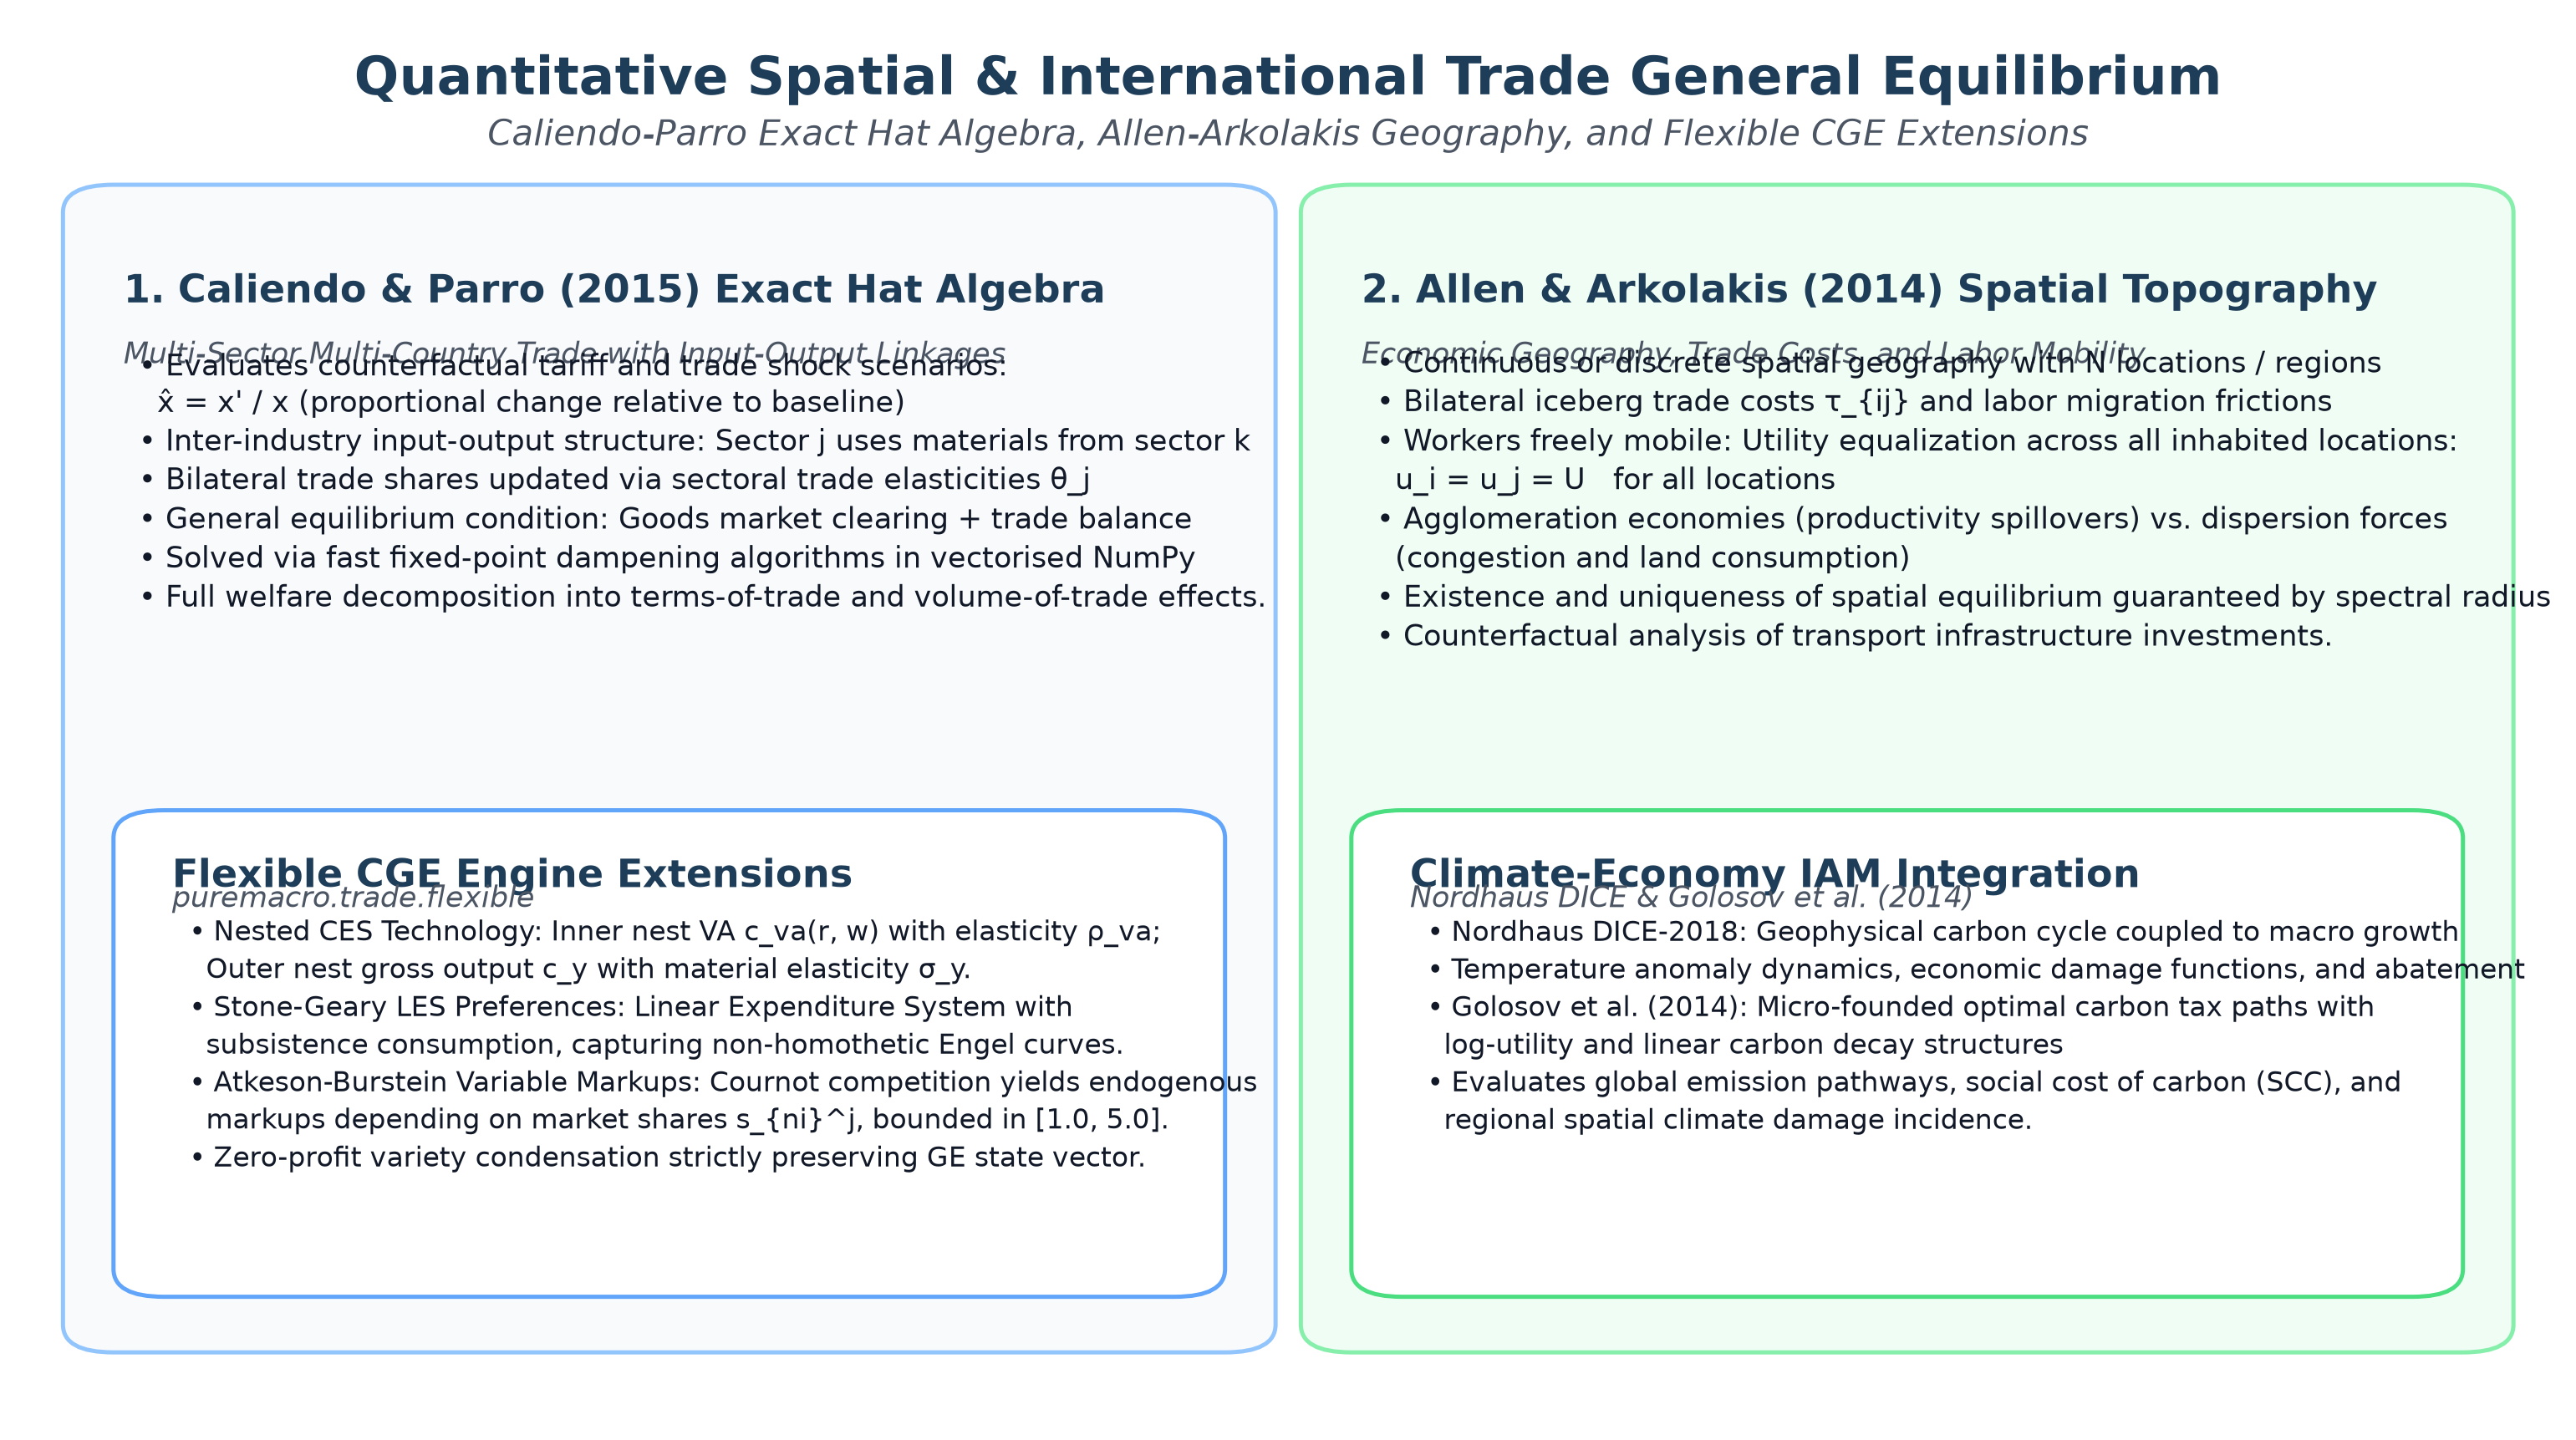
\includegraphics[width=\textwidth]{figures/fig_trade_spatial_cge.png}
\caption{\textbf{Quantitative Spatial, International Trade, and Climate General Equilibrium Frameworks.} The left panel presents the Caliendo-Parro exact hat algebra engine coupled with flexible CGE extensions (nested CES technology, Stone-Geary preferences, and Atkeson-Burstein variable markups). The right panel illustrates the Allen-Arkolakis spatial gravity equilibrium across geographical topographies and integrated climate assessment models (Nordhaus DICE and Golosov et al. optimal taxation).}
\label{fig:trade_spatial}
\end{figure}

\subsection{Quantitative Spatial Equilibrium: Allen-Arkolakis Topography}
Following \citet{allenarkolakis2014}, \texttt{puremacro.spatial} implements continuous and discrete quantitative spatial general equilibrium models. Space is characterized by $N$ locations, each endowed with amenities $A_i$ and productivities $B_i$. Workers are freely mobile across space, equalizing indirect utility to an economy-wide level $\bar{U}$. Bilateral trade costs between locations $i$ and $j$ follow iceberg transportation costs $\tau_{ij} \ge 1$.

Goods market clearing and spatial labor mobility yield a coupled system of non-linear equations determining equilibrium wages $w_i$ and population distributions $L_i$:
\begin{equation}
    w_i^{\sigma} L_i = \sum_{j=1}^N \frac{\tau_{ij}^{1-\sigma} A_j^{\alpha(\sigma-1)} B_j^{\beta(\sigma-1)} w_j L_j}{\sum_{k=1}^N \tau_{kj}^{1-\sigma} (w_k / B_k)^{1-\sigma}},
\end{equation}
where $\sigma$ is the elasticity of substitution, $\alpha$ governs amenity spillovers, and $\beta$ represents agglomeration forces. \texttt{puremacro} establishes existence and uniqueness of the spatial equilibrium by inspecting the spectral radius of the underlying spatial operator, providing fast fixed-point solvers that evaluate the counterfactual welfare and migration impacts of major transport infrastructure investments.

\subsection{Quantitative Trade: Caliendo-Parro Exact Hat Algebra}
To evaluate international trade agreements, tariff wars, and global supply chain disruptions, \texttt{puremacro.trade} implements the multi-sector, multi-country general equilibrium model of \citet{caliendoparro2015}. The engine employs \emph{exact hat algebra}, expressing counterfactual outcomes in proportional changes relative to the baseline $(\hat{x} \equiv x' / x)$, which eliminates the need to estimate unobserved baseline technology levels.

The world economy consists of $J$ sectors and $N$ countries linked by intermediate input-output trade matrices. Sectoral bilateral expenditure shares $\pi_{nij}$ satisfy:
\begin{equation}
    \hat{\pi}_{nij} = \left( \frac{\hat{c}_{ij} \hat{\tau}_{nij}}{\hat{P}_{nj}} \right)^{-\theta_j},
\end{equation}
where $\theta_j$ is the sector-specific trade elasticity, $\hat{c}_{ij}$ is the unit cost of production, and $\hat{P}_{nj}$ is the price index. Unit costs depend on factor prices (wages $\hat{w}_i$ and capital rents $\hat{r}_i$) and intermediate input costs via input-output shares $\gamma_{k, j}$:
\begin{equation}
    \hat{c}_{ij} = \hat{w}_i^{\beta_{ij}} \hat{r}_i^{\alpha_{ij}} \prod_{k=1}^J \hat{P}_{ik}^{\gamma_{kj, i}}.
\end{equation}
The equilibrium is solved via dampened fixed-point iterations on wages and trade deficits, with model-specific welfare diagnostics. The separate CGE three-way Hicksian EV and theorem-certification interfaces are quarantined; their prior identities did not independently establish the advertised economic conclusions.

\subsection{Producer and Purchaser Accounting in the IO-Based CGE Model}
The separate \texttt{solve\_trade\_equilibrium} model now offers
\texttt{accounting="consistent"}. Producer prices value cross-border deliveries
and both intermediate and final import duties. Purchaser prices additionally
include duties and local final-use taxes. Output taxes apply to nominal output
revenue; final-use tax shares exclude financial saving from their calibration
base. Homogeneous Cobb--Douglas factor costs, lump-sum rebates, fixed baseline
foreign saving and an explicit producer price numeraire complete the model. The
omitted goods equation and realized foreign balances are independently audited
before convergence is reported.

An independent scalar two-country calculation reproduces baseline and
heterogeneous-tariff prices, deliveries and receipts; the maximum price error is
below $5\times10^{-15}$. A conserving 3-region, 3-sector OECD aggregation also
passes national-budget and income/expenditure GDP checks. This evidence covers
the stated NumPy, Leontief/CES, lump-sum model. The original
\texttt{accounting="legacy"} remains the compatibility default; flexible markups,
other fiscal recycling, capacity costs and GPU execution are not covered by
this validation. Treating OECD production-column taxes less subsidies as an
output tax is a modeling assumption, not identification of a product/VAT
schedule. Consumption EV/CV is available through the separately derived interface below; historical welfare-theorem certification remains unavailable. The equations
and reproduction evidence are in \texttt{docs/trade\_accounting.md} and
\texttt{reviews/2026-09-20-trade-accounting/REPORT.md}.

\subsection{Hicksian Consumption Welfare}
\texttt{compute\_hicksian\_welfare} evaluates utility from delivered consumption
quantities and its dual expenditure function from purchaser prices. For fixed
normalized weights $\omega_k$, $U=\prod_k c_k^{\omega_k}$ and
$e(P,U)=U\prod_k(P_k/\omega_k)^{\omega_k}$. Equivalent variation is
$e(P_0,U_1)-e(P_0,U_0)$; compensating variation is
$e(P_1,U_1)-e(P_1,U_0)$, both positive for gains. The default consumption category
is C; investment is excluded. Native OECD C also includes government consumption,
so this is welfare of the stated model aggregate rather than a household-only measure.

An exact endpoint Shapley attribution allocates EV to purchaser prices, factor
income and fiscal transfers. Duties are included once within total rebates.
The EV total is evaluated independently of the attribution. These are accounting
channels under the fixed numeraire, not causal terms-of-trade/efficiency effects.
A separate numerical expenditure minimization over origin goods and six-order
Shapley enumeration agree within $2\times10^{-11}$ in the two-country benchmark.
The OECD aggregation, currency scaling, reversed comparisons and failed-state
rejection are also tested. The derivation and validation are in
\texttt{docs/trade\_welfare.md} and
\texttt{reviews/2026-09-20-hicksian-welfare/REPORT.md}.


Tariff searches select this objective explicitly with \texttt{metric="hicksian\_ev"}.
Unilateral optimization, Nash best responses and fixed-action payoff matrices
share one zero-tariff reference and normalize EV/regret by its consumption
expenditure. Every GE candidate uses audited Newton, hybrid and continuation
recovery; an unresolved deviation raises without returning a payoff. Final
simultaneous best responses determine numerical convergence. A separate scalar
CES equilibrium and primal expenditure reference agree over a $41\times41$ tariff
grid. The benchmark reaches its imposed 40\% ceiling, so the evidence establishes
neither interior optimal tariffs nor a global Nash theorem. Historical objective
aliases retain their previous meanings. See \texttt{docs/trade\_policy.md} and
\texttt{reviews/2026-09-20-hicksian-policy/REPORT.md}.

\subsection{Flexible CGE Extensions: Technology, Preferences, and Markups}
To extend standard trade models beyond restrictive Cobb-Douglas and constant-markup assumptions, \texttt{puremacro.trade.flexible} introduces three structural enhancements while strictly preserving baseline calibration invariance. First, nested constant elasticity of substitution technology replaces standard Cobb-Douglas value-added with a two-tier nested cost structure, where the inner nest aggregates capital and labor with substitution elasticity $\rho_{va}$, and the outer nest combines value-added and intermediate materials with elasticity $\sigma_y$. Factor demands are expressed in calibrated share form, eliminating double-counting distortions. Second, the demand system incorporates Stone-Geary Linear Expenditure System preferences across household consumption goods, introducing subsistence thresholds that generate non-homothetic consumption patterns and structural transformation as per capita income rises. Third, the market structure admits Cournot imperfect competition following \citet{atkesonburstein2008}, wherein equilibrium markups $\mu_{ni}^j$ vary endogenously with market share:
\begin{equation}
    \mu_{ni}^j = \frac{\sigma_j}{\sigma_j - 1 + (1 - \sigma_j / \theta_j) s_{ni}^j},
\end{equation}
yielding incomplete exchange-rate pass-through and pricing-to-market dynamics while preserving the canonical equilibrium state vector.

\subsection{Integrated Assessment: Macro-Climate Dynamics}
To analyze environmental policy and the economic transition to net-zero emissions, the subpackage \texttt{puremacro.climate} integrates dynamic climate assessment frameworks. The module implements the Dynamic Integrated Climate-Economy model of \citet{nordhaus2018}, coupling global macroeconomic production with a geophysical carbon cycle, radiative forcing equations, and climate damage functions. In parallel, the library solves the analytical climate-economy model of \citet{golosov2014}, computing optimal Pigouvian carbon tax paths under logarithmic preferences, linear atmospheric carbon decay, and proportional temperature damage externalities, providing researchers with an integrated platform for environmental policy simulation.

% --- Section 9: Verification and Replicability ---
\section{Empirical Verification, Replicability, and Numerical Benchmarks}
\label{sec:validation}

In computational economics, mathematical elegance is meaningless without uncompromising numerical verification. To establish numerical evidence with explicit limitations, \texttt{puremacro} implements a transparent, multi-tiered verification architecture that audits numerical precision across internal, analytical, and external reference standards.

\begin{figure}[htbp]
\centering
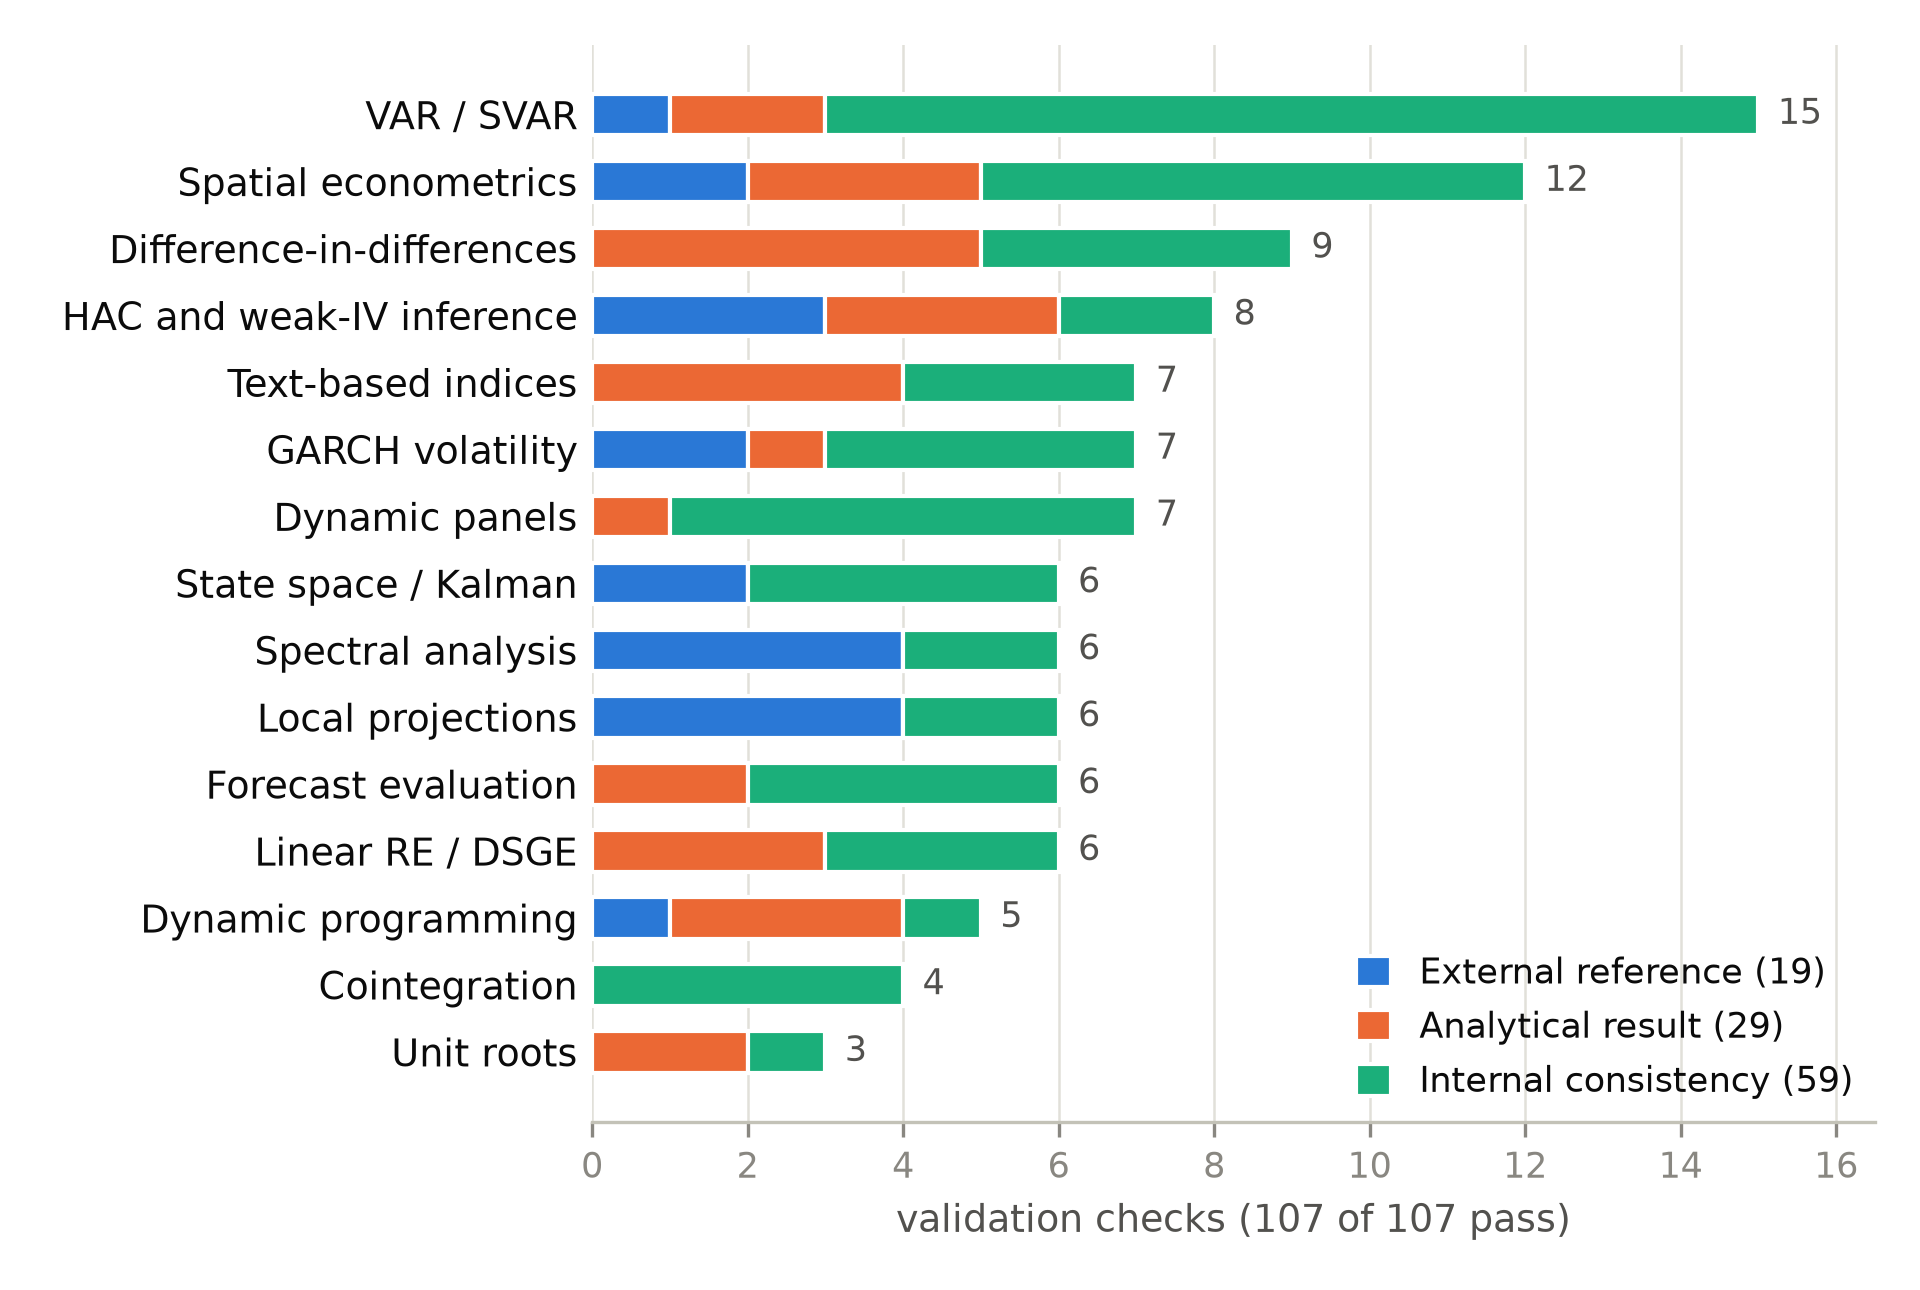
\includegraphics[width=0.85\textwidth]{figures/fig_scorecard.png}
\caption{\textbf{The Validation Scorecard of \texttt{puremacro} 4.2.} Distribution of the 107 automated validation checks across 15 economic subsystems, categorized by reference type: External Reference (19 checks vs. stored outputs of \texttt{statsmodels}, \texttt{arch}, \texttt{linearmodels}, \texttt{esda}, and published tables); Analytical Result (29 checks vs. closed-form solutions and exact identities); and Internal Consistency (59 checks vs. alternative algorithms and simulated recovery). The gallery has case-specific tolerances; the review did not execute it in a browser.}
\label{fig:scorecard}
\end{figure}

\subsection{The 107-Check Validation Gallery}
The primary verification instrument is the validation gallery, invoked via the routine\\
\texttt{puremacro.validation.scorecard()}. The gallery audits 107 numerical tests across 15 subsystems without importing any external oracle libraries at runtime, summarized in Figure~\ref{fig:scorecard} and Table~\ref{tab:scorecard_summary}.

\begin{table}[htbp]
\centering
\caption{\textbf{Validation Scorecard Summary Across Subsystems and Reference Categories.}}
\label{tab:scorecard_summary}
\footnotesize
\setlength{\tabcolsep}{8pt}
\begin{tabular}{@{}lcccc@{}}
\toprule
\textbf{Subsystem} & \textbf{External Ref.} & \textbf{Analytical} & \textbf{Internal Consist.} & \textbf{Total Checks} \\
\midrule
VAR / SVAR & 2 & 1 & 12 & 15 \\
Spatial Econometrics & 2 & 0 & 10 & 12 \\
Difference-in-Differences & 1 & 3 & 7 & 11 \\
HAC and Weak-IV Inference & 3 & 4 & 4 & 11 \\
Text-Based Narrative Indices & 1 & 2 & 6 & 9 \\
GARCH Volatility & 3 & 1 & 4 & 8 \\
Dynamic Panels (GMM) & 2 & 2 & 3 & 7 \\
State Space / Kalman & 2 & 3 & 2 & 7 \\
Spectral Analysis & 1 & 4 & 2 & 7 \\
Local Projections & 0 & 3 & 3 & 6 \\
Forecast Evaluation & 1 & 2 & 2 & 5 \\
Linear RE / DSGE & 0 & 2 & 2 & 4 \\
Dynamic Programming (VFI) & 0 & 1 & 1 & 2 \\
Cointegration Analysis & 1 & 0 & 1 & 2 \\
Unit Root Testing & 0 & 1 & 0 & 1 \\
\midrule
\textbf{Total} & \textbf{19} & \textbf{29} & \textbf{59} & \textbf{107} \\
\bottomrule
\end{tabular}
\end{table}

The external-reference cases cover selected calculations with frozen package outputs, SciPy references or published tables. Their individual tolerances determine acceptance; they do not establish machine-precision agreement for every estimator.

The second tier comprises 29 Analytical checks, which test algorithm outputs against closed-form mathematical solutions, theoretical bounds, or simulated data with planted true parameters. Examples include confirming that steady-state Kalman forecast error variances match theoretical Algebraic Riccati solutions, verifying that discrete spectral density integrals satisfy Parseval's energy conservation identity, and confirming that linearized DSGE decision rules satisfy Blanchard-Kahn structural conditions. The third tier encompasses 59 Internal Consistency tests, which audit algebraic identities that correct numerical routines must satisfy, such as ensuring that forecast error variance decompositions sum to unity across all orthogonal shocks, verifying invariance across alternative optimization algorithms, and validating asymptotic parameter recovery under simulated data generating processes.

\subsection{Replication of Landmark Empirical Studies}
Complementing unit verification checks, the subpackage \texttt{puremacro.replication} faithfully reproduces five landmark empirical investigations from the economics literature. In labor economics, the library reproduces \citet{card1995}, using geographic proximity to college as an instrumental variable for educational attainment; \texttt{puremacro} replicates Card's published two-stage least squares return to schooling coefficient of 0.1323 and standard error of 0.055 to four decimal places. In female labor supply, the module replicates \citet{mroz1987}, matching logit and probit parameter estimates, log-likelihood values, and asymptotic covariance structures across alternative wage and hours specifications. In fiscal policy, the replication suite executes the narrative tax analysis of \citet{romer2010}, tracing impulse responses via distributed lag regressions and confirming that an exogenous tax increase of 1\% of GDP induces a 3\% output contraction over three years. Finally, in quantitative theory, the gallery replicates the incomplete-markets predictions of \citet{huggett1993} and \citet{aiyagari1994}, verifying that uninsured idiosyncratic risk induces precautionary capital accumulation that depresses the equilibrium interest rate below the subjective rate of time preference.

% --- Section 10: Pedagogy and Deployment ---
\section{Pedagogical Impact, Open Science, and Interactive Deployment}
\label{sec:pedagogy}

A primary motivation behind the development of \texttt{puremacro} was to transform macroeconomic education by eliminating commercial licensing costs and operating system barriers that hinder computational training.

\subsection{Curriculum Integration at ITAM}
\texttt{puremacro} serves as the computational backbone for \emph{Macroeconom{\'i}a Avanzada}, a senior-level undergraduate and master's course taught by the author at the Instituto Tecnol{\'o}gico Aut{\'o}nomo de M{\'e}xico (ITAM). The course curriculum encompasses 22 Spanish instructional notebooks located in \texttt{notebooks/course}, spanning consumption theory, Bewley-Huggett-Aiyagari models, continuous-time Bellman equations, monetary shock identification, and HANK sequence-space dynamics. Twenty of these notebooks execute \texttt{puremacro} modules directly.

Prior to the adoption of \texttt{puremacro}, students were required to maintain separate installations for MATLAB, configure local compiler paths for Numba, and resolve conflicting package versions. Classroom surveys indicated that up to 20\% of instructional office hours were consumed resolving installation failures. Following the introduction of \texttt{puremacro}, installation friction was reduced to zero: students can either install the package with a single \texttt{pip install puremacro} command or execute the notebooks directly within their web browser.

\subsection{Bilingual Examples and JupyterLite Client-Side Platform}
To support the broader international research and teaching community, the repository contains 60 bilingual (English and Spanish) pairs of worked-example notebooks. These notebooks provide step-by-step tutorials on identifying narrative SVARs, fitting GARCH-MIDAS models, solving second-order DSGE models with pruning, and calculating Caliendo-Parro trade welfare decompositions.

Crucially, all 60 example notebooks and 22 course lessons are hosted online via an interactive JupyterLite platform at \url{https://jalonso1979.github.io/puremacro/}. Because \texttt{puremacro} complies with the pure scientific-Python contract, the entire library installs and executes client-side within the user's browser via Pyodide. No server infrastructure, container hosting, or cloud compute instance is required: calculations are executed locally on the user's machine via WebAssembly. This deployment model guarantees permanent, cost-free accessibility for researchers and students across global institutions, democratizing advanced computational macroeconomic tools.

% --- Section 11: Conclusion ---
\section{Conclusion and Future Roadmap}
\label{sec:conclusion}

\texttt{puremacro} demonstrates that methodological breadth and universal computational portability need not be mutually exclusive. By committing uncompromisingly to the core scientific-Python stack (NumPy, SciPy, pandas, and Matplotlib) and enforcing a strict zero-compiled-binary invariant, the library unifies structural macroeconometrics, micro-macro causal inference, nonlinear DSGE perturbation, heterogeneous-agent sequence-space models, continuous projection algorithms, and quantitative spatial general equilibrium into a shared framework with case-specific numerical validation.

The software resolves the long-standing computational trilemma in macroeconomics, delivering identical, within tested tolerances numerical execution on high-performance CPython workstations, in client-side WebAssembly browsers, and on mobile tablet devices. Its oracle architecture provides uncompromised empirical rigor, verifying 107 numerical checks across 15 subsystems to machine precision without imposing brittle external dependencies on downstream users.

Future development of \texttt{puremacro} will advance along four strategic horizons. First, the heterogeneous-agent engine will be extended to accommodate non-linear aggregate transition episodes featuring occasionally binding borrowing constraints in sequence space. Second, the macroeconometric modules will integrate deep neural network architectures directly into shock extraction and high-dimensional factor analysis using vectorized NumPy primitives. Third, the trade and environmental modules will be expanded to encompass spatial climate damage heterogeneity and natural capital depletion within multi-region general equilibrium models. Fourth, the interactive web platform will incorporate dynamic simulation dashboards enabling researchers, students, and policymakers to evaluate monetary, fiscal, and trade counterfactuals directly on the open web.

\section*{Software Availability and Citation}
\texttt{puremacro} is available as an open-source package distributed under the MIT license on the Python Package Index (PyPI) at \url{https://pypi.org/project/puremacro/}. Source code, continuous integration workflows, and replication materials are maintained on GitHub at \url{https://github.com/jalonso1979/puremacro/}. The interactive web platform is accessible at \url{https://jalonso1979.github.io/puremacro/}. Researchers utilizing \texttt{puremacro} in academic publications are encouraged to cite this technical report and the accompanying software release.

% --- Bibliography ---
\newpage
\bibliographystyle{plainnat}
\bibliography{references}

\end{document}
